\documentclass[10pt,a4paper,twoside]{report}
\usepackage[a4paper,inner=3.5cm,outer=2.5cm,top=2.5cm,bottom=2.5cm]{geometry}
\linespread{1.3} %interlinia 1.5
\setlength{\parindent}{1.25cm}
\usepackage{indentfirst}

\usepackage[utf8]{inputenc}
\usepackage{polski}
\usepackage[polish]{babel}
\usepackage{pdfpages}

\usepackage[titletoc,title]{appendix}
\usepackage{titlesec}
\usepackage{uarial}
\renewcommand*{\familydefault}{\sfdefault}

%*************
\usepackage{newtxtext, newtxmath} %lepiej wyglądające nagłówki
\usepackage{epstopdf} %do dołączania obrazków w formacie eps
\usepackage[hidelinks=true]{hyperref} % hiperłącza wewnętrzne (cytowania, odnośniki do obrazków, równań)
\usepackage{xcolor,listings} %listingi 
\usepackage[font=small,labelfont=bf]{caption} %ustawienie czcionki 9pt na podpisach
\captionsetup[table]{justification=justified,singlelinecheck=false, format=hang} %ustawienie podpisów tabel 
\usepackage{enumitem} %to, czego brakowało przy symbolach
\usepackage{algorithm}
\usepackage{algpseudocode}
\usepackage{caption}
\usepackage{subcaption}
%*************

\titleformat{\chapter}[hang]
{\normalfont\fontsize{12}{15}\bfseries\uppercase}{\thechapter.}{1em}{}
\titlespacing*{\chapter}{0pt}{12pt}{6pt}

\titleformat{\section}[hang]
{\normalfont\fontsize{10}{12}\bfseries\itshape}{\thesection.}{0.5em}{}
\titlespacing*{\section}{0pt}{12pt}{6pt}

\titleformat{\subsection}[hang]
{\normalfont\fontsize{10}{12}\itshape}{\thesubsection.}{0.5em}{}
\titlespacing*{\subsection}{0pt}{12pt}{6pt}

%%%%%%%%%%%%%%%%%%%%%%%%%%%%%%%%%%
%Formatowanie listingow
\usepackage{ucs}
\lstset{
        language=XML,
    inputencoding=utf8x, 
    extendedchars=\true,
    literate={ą}{{\k{a}}}1
             {Ą}{{\k{A}}}1
             {ę}{{\k{e}}}1
             {Ę}{{\k{E}}}1
             {ó}{{\'o}}1
             {Ó}{{\'O}}1
             {ś}{{\'s}}1
             {Ś}{{\'S}}1
             {ł}{{\l{}}}1
             {Ł}{{\L{}}}1
             {ż}{{\.z}}1
             {Ż}{{\.Z}}1
             {ź}{{\'z}}1
             {Ź}{{\'Z}}1
             {ć}{{\'c}}1
             {Ć}{{\'C}}1
             {ń}{{\'n}}1
             {Ń}{{\'N}}1
}

\lstset{
    showstringspaces=false
}

% PYTHON
\lstset{
    language=python,
    numbers=left
}

\lstdefinelanguage{JavaScript}{
    keywords={break, case, catch, continue, debugger, default, delete, do, else, finally, for, function, if, in, instanceof, new, return, switch, this, throw, try, typeof, var, void, while, with},
    morecomment=[l]{//},
    morecomment=[s]{/*}{*/},
    morestring=[b]',
    morestring=[b]",
    sensitive=true
}

%%%%%%%%%%%%%%%%%%%%%%%%%%%%%%%%%%
%Źródła w podpisach
\newcommand{\source}[1]{\vspace{-12pt} \caption*{Źródło: {#1}} }

%%%%%%%%%%%%%%%%%%%%%%
%Zamiana chapter na rozdział
\addto\extraspolish{%
    \renewcommand{\chapterautorefname}{rozdziale}%
    \renewcommand{\sectionautorefname}{podrozdziale}%
    \renewcommand{\subsectionautorefname}{sekcja}%
}
\begin{document}

\chapter*{Streszczenie}

W pracy przedstawiono dwa algorytmy mające służyć do wykrywania powierzchni w danych LiDAR.
Dzięki wykryciu powierzchni możliwa jest zamiana chmury punktów na dane wektorowe, tym samym
zmniejszenie objętości zajmowanej przez dane nawet 100-krotnie. Prezentowanie tak zmienionych danych
możliwe jest przez sieć Internet. Przedstawiono sposób zamieniania danych, a także wyniki eksperymentów.


\bigskip

\noindent\textbf{Słowa kluczowe:} LiDAR

\bigskip

\noindent\textbf{Dziedzina nauki i techniki zgodna z OECD} Nauki inżynieryjne i techniczne

\chapter*{Abstract}

Lorem ipsum dolor sit amet, consectetuer adipiscing elit, sed diam nonummy nibh euismod tincidunt ut laoreet dolore magna aliquam erat volutpat. Ut wisi enim ad minim veniam, quis nostrud exerci tation ullamcorper suscipit lobortis nisl ut aliquip ex ea commodo consequat. Duis autem vel eum iriure dolor in hendrerit in vulputate velit esse molestie consequat, vel illum dolore eu feugiat nulla facilisis at vero eros et accumsan et iusto odio dignissim qui blandit praesent luptatum zzril delenit augue duis dolore te feugait nulla facilisi. Nam liber tempor cum soluta nobis eleifend option congue nihil imperdiet doming id quod mazim placerat facer possim assum. Typi non habent claritatem insitam; est usus legentis in iis qui facit eorum claritatem. Investigationes demonstraverunt lectores legere me lius quod ii legunt saepius. Claritas est etiam processus dynamicus, qui sequitur mutationem consuetudium lectorum. Mirum est notare quam littera gothica, quam nunc putamus parum claram, anteposuerit litterarum formas humanitatis per seacula quarta decima et quinta decima. Eodem modo typi, qui nunc nobis videntur parum clari, fiant sollemnes in futurum.

\bigskip

\noindent\textbf{Keywords:} lorem ipsum, ...

\bigskip

\noindent\textbf{OECD consistent field of science and technology classification:} Nauki inżynieryjne i techniczne


\tableofcontents
\addcontentsline{toc}{chapter}{Spis treści}

\chapter*{Wykaz wa\.zniejszych oznacze\'n i skrótów}

\begin{description}[noitemsep,topsep=0pt,parsep=0pt,partopsep=0pt,labelwidth=1cm,align=left,itemindent=0pt]
    \item[CHM] - Canopy Height Model
    \item[DSM] - Digital Surface Model
    \item[DTM] - Digital Terrain Model
    \item[GEOBIA] - Geographic-Object-Based Image Analysis
    \item[GIS] - System Informacji Geograficznej (Geographic Information System)
    \item[GLONASS] - Globalnaja Nawigacionnaja Sputnikowaja Sistiema
    \item[GML] - Geography Markup Language
    \item[GPS] - Global Positioning System
    \item[HMM] - Hidden Markov Model
    \item[HTTP] - Hypertext Transfer Protocol
    \item[INS] - Inertial Navigation System
    \item[ISO] - International Organization for Standardization
    \item[ISOK] - Informatyczny System Ochrony Kraju
    \item[KML] - Keyhole Markup Language
    \item[LiDAR] - Light Detection and Ranging
    \item[LRF] - Laser Rangefinder
    \item[MB] - Megabajt
    \item[OBIA] - Object-based Image Analysis
    \item[OGC] - Open Geospatial Consortium
    \item[PCA] - Principal Component Analysis
    \item[RGB] - Red Green Blue
    \item[SHP] - Shapefile
    \item[SVM] - Support Vector Machine
    \item[TB] - Terabajt
    \item[TIN] - Triangulated Irregular Network
    \item[WCF] - Web Coverage Service
    \item[WFS] - Web Feature Service
    \item[WMS] - Web Map Service
    \item[XML] - Extensible Markup Language
\end{description}


\chapter{Wst\k{e}p i cel pracy}

Jeszcze kilkadziesiąt lat temu jedynym źródłem wiedzy na temat otaczającej przestrzeni były mapy.
Ze względu na ich charakter oraz szybkie tempo rozwoju (np: infrastruktury drogowej) deaktualizowały
się bardzo szybko. Co więcej, nie zawierały one informacji dotyczących ukształtowania powierzchni.
Oczywiście, poprzez system poziomic możliwe jest określnie wysokości danego punktu, jedakże wiąże się to
z pewną niedokładnością oraz wymaga się, aby punkt znajdował się na powierzchni Ziemi. Brakuje
map analogowych, zawierających informację o wysokości budynków. Tworzyło to wrażenie niedostatku informacji.

Wraz z rozwojem lotnictwa, a następnie satelit kosmicznych, sytuacja zaczęła sie odwracać. Powstawały coraz to
nowe metody zbierania informacji dotyczących powierzchni ziemi. W dzisiejszym świecie, dzięki istnieniu aplikacji
takich jak Google Maps, możemy zobaczyć nie tylko mapę dowolnego miejsca na Ziemi,
ale też obejrzeć zdjęcia lotnicze danego terenu a nawet panoramę z poziomu ulicy. Rozwinęła się też nawigacja - dzięki powstaniu
systemów: amerykańskiego GPS\cite{website:gps}, rosyjskiego GLONASS\cite{website:glonass}, a w późniejszym czasie - chińskiego Baidu oraz europejskiego Galileo możliwe
jest ustalenie pozycji w czasie rzeczywistym z dokładnością do kilku centymetrów. Ponadto odbiorniki GNSS są niezwykle tanie i
powszechne - można je znaleźć w niemal każdym nowoczesnym smartfonie.
Jednocześnie istnieją projekty badawcze, takie jak
\textit{Copernicus}\cite{webiste:copernicus} który zbiera dane za pomocą radarów SAR czy \textit{ISOK}\cite{website:isok} który zbiera
dane LiDAR.

Rozwija się też sama aparatura badawcza. Dzisiejsze smartfony wykonują zdjęcia w rozdzielczości niedostępnej w najdroższych
aparatach sprzed kilkudziesięciu lat. Rośnie też rozdzielczość danych zbieranych w pasmach innych niż widzialne.
Także dane LiDAR są wykonywane w coraz większej rozdzielczości, sięgającej nawet kilkudziesięciu punktów na metr kwadratowy.

Widać wyraźnie, iż diametralnie rośnie ilość pozyskiwanych danych przestrzennych. Nie tylko zwiększa się ilość urządzeń
pomiarowych (satelity, samoloty) ale też sama ilość informacji pozyskiwana z jednego urządzenia. Stawia to nowe wyzwania przed badaczami,
którzy te ogromne ilości danych muszą przetworzyć i udostępnić w przyjazny sposób dla użytkownika.

Szczególnie wymagające jest udostępnianie danych LiDAR w wysokiej rozdzielczości ze względu na ich rozmiar. Plik zawierający
w sobie dane dotyczące obszaru wielkości około $0,35km^2$ zajmuje 180MB. Przesłanie takiego pliku przez sieć Internet wymaga
czasu kliku, czasem nawet kilkunastu sekund. Stąd też pojawia się idea, aby dane te uprościć, a tym samym zmniejszyć czas potrzebny
na ich przesłanie przez sieć

\section{Cele i teza pracy}

Głównym celem pracy jest stwierdzenie, czy możliwe jest stworzenie systemu który umożliwi dostęp do danych zebranych za pomocą
skanowania laserowego w formie mapy cyfrowej. Aby potwierdzić lub zaprzeczyć tezie zostaną zaimplementowane różne algorytmy, których
zadaniem będzie możliwie bezstratna kompresja danych LiDAR. Kompresja będzie polegać na odnajdowaniu specyficznych grup punków, które
w rzeczywistości stanowią fragment tej samej powierzchni. Po zalezieniu otoczki takiej powierzchni, możliwe będzie odrzucenie punktów
znajdujących się w jej środku i pozostawienie tylko wielokąta o kształcie tejże powierzchni, tym samym zmniejszając ilość danych
koniecznych do przesyłania

\section{Przegląd rozdziałów}

W rozdziale drugim zostały omówione sposoby pozyskiwania danych LiDAR.
Następnie omówiono rózne algorytmy stosowane w celu przetwarzania chmury punktów.

W rozdziale trzecim omówiono technologie stosowane podczas przesyłania danych geograficznych przez sieć. Rozpoczynając od protokołów,
poprzez usługi serwerowe dostarczające mapy kończąc na bibliotekach klienckich pozwalających przeglądać te dane.

W rozdziale czwartym przedstawiono dwa zaimplementowane algorytmy. Omówiono ich zasadę działania oraz wskazano na różnicę między nimi.
Dodatkowo opisano w jaki sposób przekształca się dane do formatu SHP.

W rozdziale piątym przedstawiono wyniki eksperymentów przeprowadzonych zarówno na spreparowanych danych jak i na pochodzących z prawdziwego
skanowania laserowego. Porównano jakość uzyskanych wyników a także czasy przetwarzania.

W rozdziale szóstym przedstawiono ostateczne wnioski z pracy.

\chapter{Algorytmy przetwarzania chmur punktów w systemach GIS}

\section{Pozyskiwanie danych}
Do pozyskiwania danych wykorzystuje się technologię LIDAR. Jest to nowoczesna metoda pozyskiwania informacji dotyczących wysokości terenu \cite{Marmol2003}. Efektem jej działania jest tzw “chmura punktów”, która uwzględnia wysokość nie tylko powierzchni ziemi, ale również drzew, budynków itp.

Dane zbierane są za pomocą aparatury umieszczonej w samolotach, na którą składają się odbiornik GPS służący do określania pozycji, czujnik INS pozwalający na określenie aktualnego przechyłu pojazdu oraz laser LRF mierzący odległość \cite{WBPW2012}. Laser emituje wiązkę w kierunku ziemi. Na podstawie czasu jaki minął między emisją wiązki a jej odczytem, określana jest odległość między aparaturą a badanym punktem. Jednocześnie zapisywane jest położenie skanera, co pozwala umieścić punkt w układzie odniesienia (np: WGS 84).

Urządzenia LIDAR pozwalają na rejestrację niemal dowolnych ilości tzw. impulsów pośrednich, które pochodzą np: od drzew. Dzięki temu chmura punktów pochodząca z jednego przelotu może posłużyć zarówno do utworzenia numerycznego modelu pokrycia terenu, jak również do utworzenia numerycznego modelu rzeźby terenu.

\begin{figure}[h!]
\centering
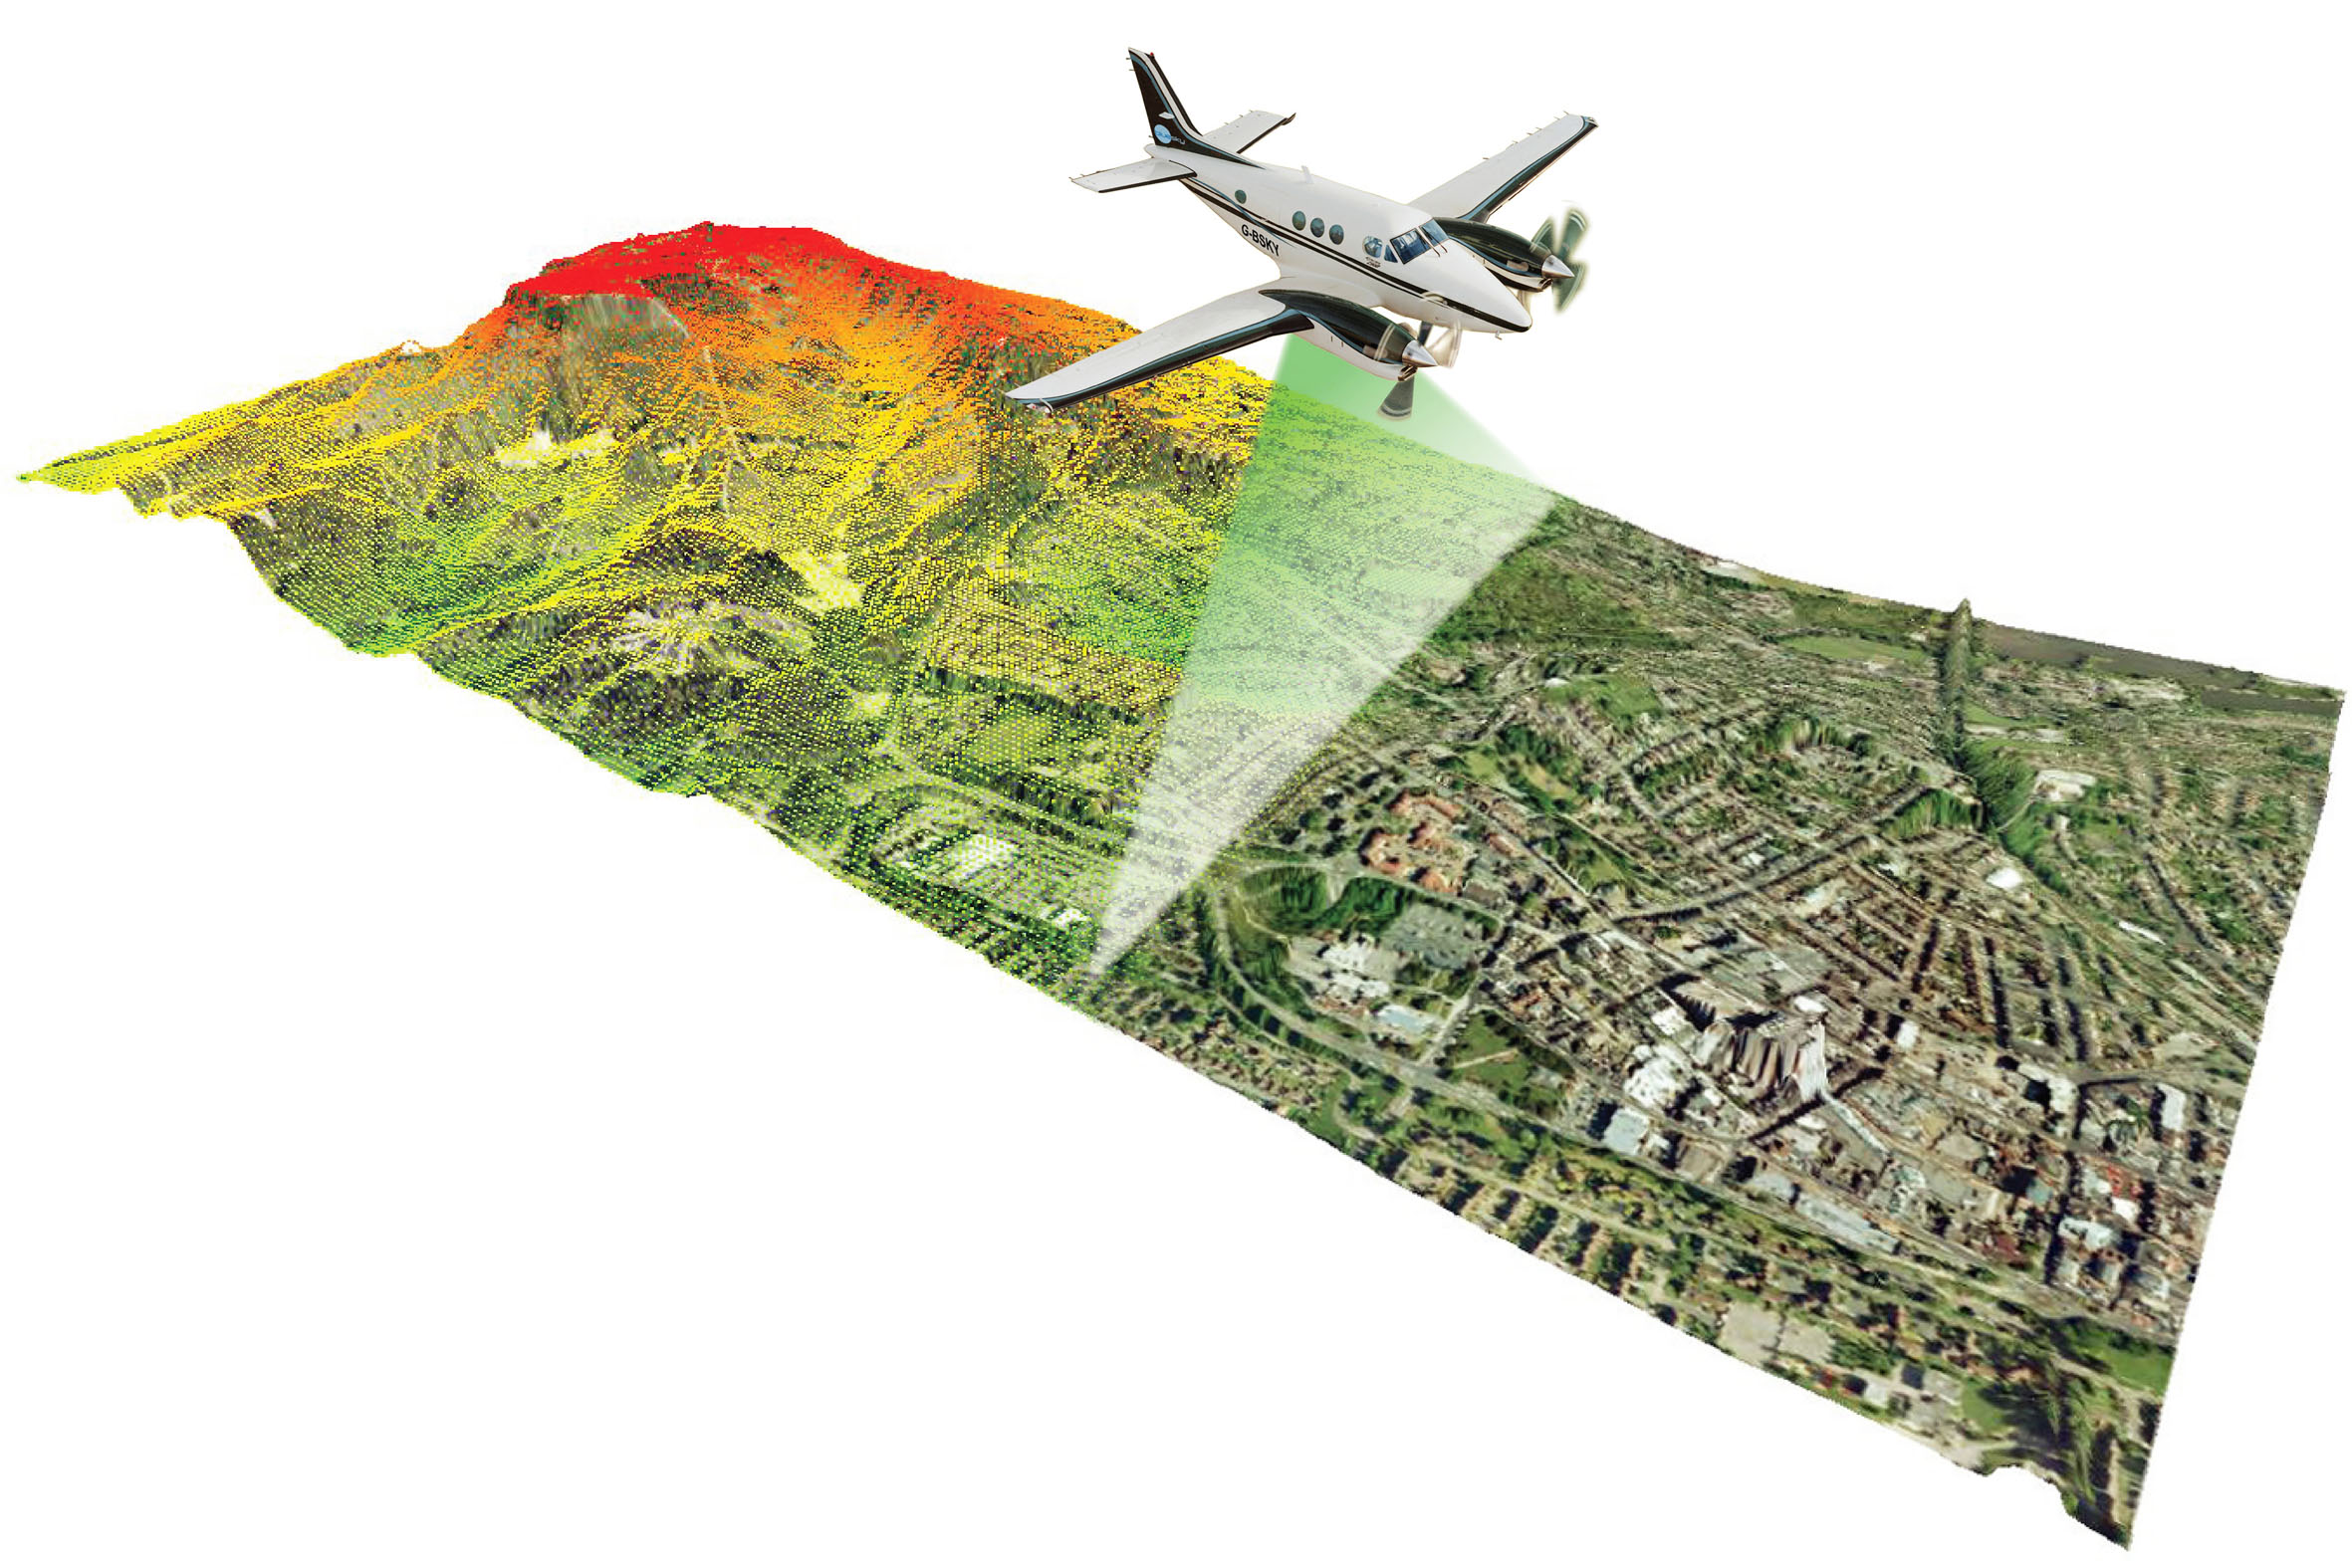
\includegraphics[width=1\textwidth]{img/LIDAR.jpg}
\caption{Schematycznie przedstawiony nalot podczas zbierania danych LIDAR}
\label{fig:lidar}
\end{figure}

Na rysunku \ref{fig:lidar} przedstawiono w sposób schematyczny jak przebiega pobieranie danych. Samolot podczas nalotu pobiera dane wzdłuż pewnego odcinka prostopadłego do kierunku lotu, z których następnie powstaje chmura punktów, której wizualizację również przedstawiono na rysunku.

\section{Opis wybranych algorytmów}

W poniższym rozdziale zostaną opisane istniejące algorytmy przetwarzania danych w postaci chmury punktów w systemach GIS.

\subsection{Triangulacja Delaunay'a}

\subsubsection{Definicja}
Triangulacja Delaunay'a jest reprezentacją chmury punktów w postaci nieregularnej siatki trójkątów TIN (z ang. Triangulated Irregular Network).
Jej cechą szczególną jest fakt, iż żaden z punktów nie leży wewnątrz okręgu opisanego na dowolnym trójkącie \cite{Lee1980}. Podział ten ma tę własność, że maksymalizuje najmniejszy kąt spośród 
wszystkich trójkątów należących do triangulacji. Na rysunku \ref{fig:triangulacja} przedstawiono przykładową triangulacje.

\begin{figure}[h!]
    \centering
    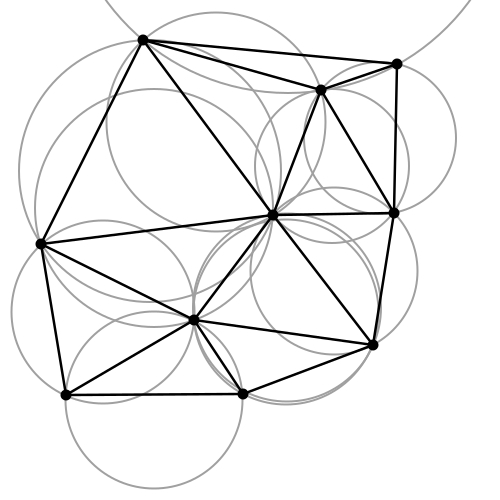
\includegraphics[width=0.5\textwidth]{img/triangulacja.jpg}
    \caption{Triangulacja Delaunay z zaznaczonymi okręgami opisanymi na trójkątach}
    \label{fig:triangulacja}
\end{figure}

\subsubsection{Aplikacje}
Triangulacja Delaunay'a jest często wykorzystywana przy przetwarzaniu danych LIDAR. Dzięki stosowaniu filtracji może służyć do oddzielania poszczególnych zbiorów punktów od siebie \cite{koziol2007} bądź też do znajdywania łamanej otaczającej zadany zbiór punktów \cite{website:HumanGeoBlog}. Istnieje wiele implementacji algorytmu pozwalającego na przetworzenie chmury punktów do postaci siatki trójkątów \cite{Lee1980,Dwyer1987,jiang2010}. W artykule \cite{Lee1980} opisano dwa algorytmy tworzenia takiej siatki - dziel i zwyciężaj oraz tribuild. Pierwszy z nich o złożoności obliczeniowej $O(N log N)$ rekurencyjnie dzieli zbiór punktów pośrednich na mniejsze zbiory, w nich dokonuje triangulacji a następnie łączy je. Drugi z nich o złożoności obliczeniowej $O(N^{3/2})$ zakłada znajomość prostokąta który otacza zadany zbiór punktów. Prostokąt ten jest dzielony na mniejsze, a następnie dla każdego mniejszego prostokąta:

\begin{algorithmic}
    \For {punkt P w punktach należących do prostokąta}
    \If {P jedyny punkt w prostokącie}
        \State połącz punkt z wierzchołkami prostokąta
    \Else
        \State dodaj krawędzie, aby nie zniszczyć triangulacji
    \EndIf
    \EndFor
\end{algorithmic}

Przykładowe kolejne etapy tak przeprowadzonej triangulacji pokazano na rysunku \ref{fig:iter_triangulacja}.

\begin{figure}[h!]
    \centering
    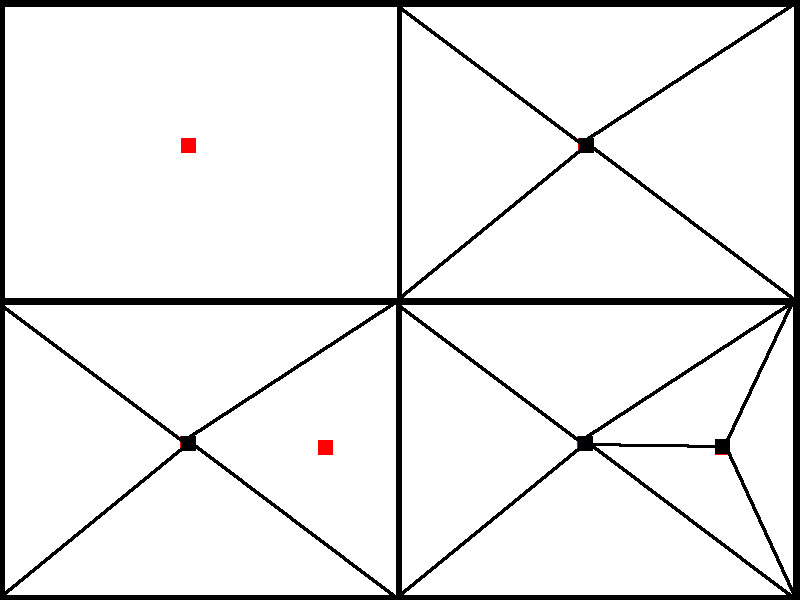
\includegraphics[width=0.5\textwidth]{img/iter_triangulacja.jpg}
    \caption{Iteracyjna triangulacja}
    \label{fig:iter_triangulacja}
\end{figure}

W 1987 Dwayer zaproponował szybszy algorytm dziel i zwyciężaj, o zakładanej złożoności $O(N log log N)$, jednak w pesymistycznym przypadku dalej będzie to $O(N log N)$  \cite{Dwyer1987}. Powstały też nowsze algorytmy pozwalające na stworzenie triangulacji. W artykule \textsl{An efficient algorithm for constructing Delaunay triangulation} autorzy zwracają uwagę, że w większości algorytmów szybko tworzy się siatkę a następnie dużo czasu poświęca się na lokalne optymalizacje, co skutkuje zwiększoną złożonością obliczeniową. Dzięki zaproponowaniu reguły prawej dłoni, udało im się znacząco zmniejszyć ilość obliczeń potrzebnych do przeprowadzenia lokalnych optymalizacji, tym samym proponowany algorytm ma złożoność na poziomie $O(N)$ \cite{jiang2010}.

\subsection{Maszyny wektorów nośnych}

\subsubsection{Definicja} 

Maszyny wektorów nośnych SVN (z ang. \textit{support vector machine}) pozwalają na rozwiązanie tzw. problemu klasyfikacji. Definicja problemu brzmi następująco: dla pewnej przestrzeni $\Omega$ zawierającej wektory danych x, należące do dwóch klas
$\Omega = \{(x_{i}, c_{i}) | x_{i} \in R^p, c_{i} \in \{-1,1\}\}$
należy znaleźć klasyfikator który podzieli tę przestrzeń na dwa rozłączne obszary jak najlepiej odpowiadające klasom $\{-1, 1\}$ \cite{stefanowski2010}. Do rozdzielenia zbioru na dwa służy tzw. liniowa funkcja separująca (lub jej uogólnienie - hiperpłaszczyzna dla przypadków n-wymiarowych), która wyznacza podział przestrzeni na dwa podobszary.

\begin{figure}[h!]
    \begin{subfigure}[b]{0.33\textwidth}
        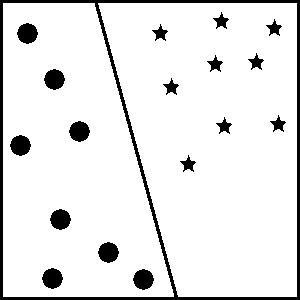
\includegraphics[width=\linewidth]{img/granica_1.jpg}
    \end{subfigure}%
    \begin{subfigure}[b]{0.33\textwidth}
        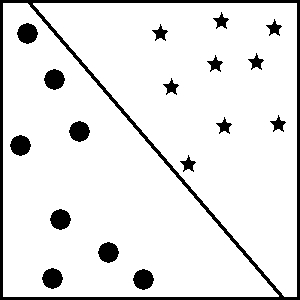
\includegraphics[width=\linewidth]{img/granica_2.jpg}
    \end{subfigure}%
    \begin{subfigure}[b]{0.33\textwidth}
        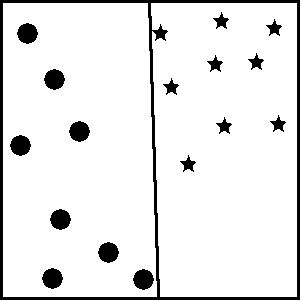
\includegraphics[width=\linewidth]{img/granica_3.jpg}
    \end{subfigure}
    \caption{Różne przykłady liniowej separacji}
    \label{fig:liniowa_separacja}
\end{figure}

Na rysunku \ref{fig:liniowa_separacja} przedstawiono różne poprawne sposoby separowania tego samego zbioru. Można w szczególności wyróżnić pary hiperpłaszczyzn $b_{i1}$ oraz $b_{i2}$, będących równoległych do 
siebie, powstałych poprzez przesuwanie jednej hiperpłaszczyzny od punktu granicznego pierwszego zbioru do punktu granicznego drugiego zbioru (rysunek \ref{fig:rownolegla_separacja}).

\begin{figure}[h!]
    \centering
    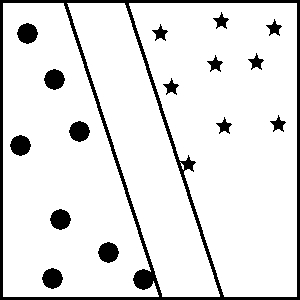
\includegraphics[width=0.33\textwidth]{img/granica_rownolegla.jpg}
    \caption{Równoległe hiperpłaszczyzny}
    \label{fig:rownolegla_separacja}
\end{figure}

Odległości pomiędzy hiperpłaszczyznami $b_{i1}$ oraz $b_{i2}$ nazywamy marginesem klasyfikatora liniowego. Maszyny wektorów nośnych znajdują taką hiperpłaszczyznę, która maksymalizuje margines. Szukamy więc hiperpłaszczyzny spełniającej warunki:

\begin{equation}
    w*x + b =0
\end{equation}

gdzie $w$ i $b$ są parametrami modelu. Wtedy przynależność do klas można wyrazić jako:

\begin{displaymath}
    y = \left\{ \begin{array}{ll}
        1 & \textrm{$w*x+b>0$}\\
        -1 & \textrm{$w*x+b<0$}\\
    \end{array} \right.
\end{displaymath}

Parametry $w$ i $b$ należy wyznaczać tak, aby maksymalne marginesy $b_{i1}$ i $b_{i2}$ były miejscem geometrycznym punktów $x$ spełniających warunki:
\begin{eqnarray}
    b_{i1} \quad w*x + b =1 \\
    b_{i2} \quad w*x + b =-1
\end{eqnarray}

\subsubsection{Aplikacje}

Możliowości wykorzystania maszyn wektorów nośnych do przetwarzania chmury punktów nasuwają się same - możliwe jest chociażby przydzielanie punktów do klas drzew i budynków \cite{xwang2011}. Istnieje wiele 
różnych przykładów na wykorzystanie SVN do przetwarzania chmur punktów \cite{xwang2011,li2013,david2015}. We wszystkich z nich część punktów pomiarowych jest wykorzystywana jako dane uczące.
Dla tych punktów operator ręcznie przydziela je do jednej z klas \cite{xwang2011}. Następnie na podstawie tych punktów możliwe jest określenie najlepszej hiperpłaszczyzny, jak opisano w sekcji \textit{definicja}.
W pracy z 2011r. wykorzystano tzw. niezbalansowane maszyny wektorów nośnych USVN (z ang. \textit{unbalanced support vector machines}) do rozróżnienia drzew i budynków \cite{xwang2011}.
Do analiz wykorzystano zdjęcia satelitarne oraz dane pochodzące z LIDARa - za pomocą tych dwóch źródeł stworzono wektory $x$ składające się z wysokości $Z$, wariancji wysokości $sZ$, różnice wysokości $hZ$,
pochodne 3-go rzędu wzdłuż osi X i Y - odpowiedno $dX$ i $dY$ - oraz wartość koloru RGB ze zdjęcia satelitarnego. 
W pracy \textit{Land classification from LiDAR full-waveforms based on multi-class support vector machines} wykorzystano SVM do przypisywania punktów do więcej niż dwóch klas \cite{li2013}. 
W innej pracy z 2015 równierz wykorzystano SVM do podziału zbioru na więcej niż dwie klasy \cite{david2015}. Analiza to posłużyła do zmierzenia powierzchni namorzyn na Filipinach. 
W tym przypadku do stworzenia wektorów $x$ wykorzystano numeryczny model powierzchmi DSM, numeryczny model terenu DTM, model wysokościowy CHM, średnią intensywność oraz ilość odbić. Co ciekawe, na podstawie
ilości odbić można określić gatunek drzewa \cite{Sasaki2012}.

\subsection{Analiza obrazu oparta obiektowo}

\subsubsection{Definicja}

Analiza obrazu oparta obiektowo OBIA (z ang. \textit{Object – based image analysis}) jest stosunkowo nową metodą \cite{burnett2003} służącą do przetwarzania obrazów. W przeciwieństwie do tradycyjnych metod przetwarzania, 
nie analizuje pojedynczych pikseli, lecz całe ich grupy, zwane obiektami. Ma to przypominać sposób, w jaki ludzie rozróżniają obiekty na zdjęciach. Jeżeli zdjęcia dotczą powierzchni ziemi (takie jak zdjęcia 
satelitarne) wyróżnia się wtedy metodę geograficznej analizy obrazu oparte obiektowo GEOBIA (z ang. \textit{Geographic Object-based Image Analysis}). Jako że tematyka całej pracy dotyczy systemów GIS,
w dalszej części będzie opisywana ten szczególny przypadek OBIA.

Metoda ta składa się z dwóch etapów. w Pierwszym z nich grupuje się podobne piksele (np. pod względem koloru) w obiekty prymitwne (prymitywy). Prymitywy służą następnie do konstruowania bardziej złożonych 
struktur, odpowiadających rzeczywistym obiektom takim jak jeziora czy drogi \cite{Blaschke2014}.  Budowanie obiektów może odbywać się stopniowo na poziome wielu wartstw, jak przedstawiono na rysunku
\ref{fig:poziomy_struktury}.

\begin{figure}[h!]
    \centering
    \includegraphics[width=0.5\textwidth]{img/obiekowa_analiza.png}
    \caption{Podział obrazu na piksele i obiekty}
    \label{fig:poziomy_struktury}
\end{figure}

\subsubsection{Aplikacje}
Metoda ta jest szeroko używana do analizy danych pochodzących ze skanowania laserowego. Jest wykorzystywana do klasyfikowania terenów miejskich \cite{zhou2013,chen2014},
wykrywania zmian powierzchni lasu \cite{zhang2014} oraz do wspomagania zarządzania terminalem kontenerowym \cite{tiede2015}. W tym ostatnim wykorzystano technikę OBIA do dokładnego określania miejsca położenia
kontenerów. Jest to zadanie o tyle łatwiejsze, iż wielkość kontenerów jest znana i podana jako norma ISO 668. Do celów analizy stworzono model DTM na podstawie danych LIDAR. Następnie do wykrywania
umiejscowie kontenerów wykorzystano dane LIDAR (pochodzące z jednego nalotu) oraz wykonywane częściej zdjęcia. Efektem jest model 3D nabrzeża.

Na polu analizy i klasyfikacji terenów miejskich metoda OBIA również odnosi sukcesy. Jednym z przykładów jest praca opisana w artkule z 2014 roku \cite{chen2014} w której autorzy za pomocą jedynie
danych LIDAR uzyskali dokładność klasfikacji punktów na poziomie  96.3\%. Wykorzystano w tym celu cztery informacje pochodzące ze skanowania - wysokość punktów nad poziomem gruntu, intensywność (czasem
nazywana amplitudą) oraz różnicę wysokości i intensywności pierwszego i ostatniego impulsu. Następnie podzielono obraz na prymitywy, jak opisano w sekcji Definicja. Na końcu nastąpiło przypisanie poszczególnych
obiektów do różnych klas na podstawie opisanych powyżej czterech atrybutów, jak przedstawia tabelka \ref{tab:przypisanie_do_klas}.

\begin{table}[h!]
    \centering
    \caption{Klasyfikacja terenów na podstawie cech}
    \label{tab:przypisanie_do_klas}
    \begin{tabular}{|c|c|c|c|}
        \hline
        Klasa & Wysokość & Intensywność & Różnica wysokości i intensywności\\
        \hline
        Trawniki & Niska & Wysoka & Bardzko niska\\
        \hline
        Trawa i roślinność & Niska & Średnia & Bardzo niska\\
        \hline
        Drogi i ziemia & Niska & Niska & Bardzo niska\\
        \hline
        Woda & Niska & Bliska 0 & Bardzo niska\\
        \hline
        Krzewy & Średnia & Średnia & Niska\\
        \hline
        Infrastruktura Publiczna & Średnia & Wysoka & Średnia\\
        \hline
        Drzewa & Duża & Wysoka & Duża\\
        \hline
        Budynki & Duża & Wysoka & Średnia\\
        \hline
    \end{tabular}
\end{table}

\section{Klasyfikacja danych}

\chapter{Technologie i systemy web-GIS}
W niniejszym rozdziale zostaną przedstawione protokoły wykorzystywane podczas serwowania map, następnie zostaną omówione serwery umożliwiające przesyłanie map (GeoServer oraz MapServer).
W ostatniej części zostaną przedstawione biblioteki klienckie mogące łączyć się z serwerami i prezentujące mapy użytkownikowi.

\section{Protokoły serwowania map - WMS, WFS, WCS}
\label{chap:protokoly}

W niniejszej sekcji zostaną opisane protokoły serwowania map:
\begin{itemize}
\item WMS - Web Map Service - standard udostępniania map w postaci rastrowej za pomocą protokołu HTTP;
\item WFS - Web Feature Service - standard udostępniania danych przestrzennych w języku znacznikowym GML;
\item WCS - Web Coverage Service - standard udostępniania zmian w danych przestrzennych w czasie.
\end{itemize}

Standardy te zostały opracowane przez Open Geospatial Consortium (OCG). Jest to międzynarodowa organizacja non-profit, skupiająca się na tworzeniu wysokiej jakości standardów dotyczących systemów GIS.

\subsection{WMS}
Web Map Service jest standardem opisującym sposób udostępniania map przez serwer w postaci rastrowej za pomocą protokołu HTTP.
Zgodnie ze standardem \cite{OpenGIS_WMS2006}, rastry te mają być generowane dynamicznie na podstawie danych geograficznych.
Mapy najczęściej są zwracane w jednym z popularnych formatów graficznych, takich jak PNG, GIF lub JPG. Rzadziej jako grafika wektorowa w formatach SVG lub WebCGM.

Standard definiuje 3 dozwolone operacje: 
\begin{enumerate}
    \item GetCapabilietes - zwraca informację opisujące serwer (m.in. jego zawartość);
    \item GetMap - zwraca mapę na podstawie zdefiniowanych parametrów geograficznych;
    \item GetFeatureInfo (opcjonalna) - zwraca informację dotyczące cech obiektów, znajdujących się na mapie.
\end{enumerate}
Wszystkie te operacje mogą być wywoływane za pomocą przeglądarki internetowej poprzez URL. Parametry, które należy podać zależą od rodzaju rządania.
W przypadku prośby o dostarczenie mapy są to np: wielkość obrazka wynikowego, część Ziemi która ma zostać zobrazowana czy odwzorowanie. Pełna lista parametrów
została przedstawiona w tabeli \ref{tab:parametry_zapytania_GetMap}. Ponadto, standard dopuszcza otrzymywanie poszczególnych map z różnych serwerów.
Tym samym, WMS umożliwia stworzenie sieci rozproszonych serwerów mapowych których klienci mogą tworzyć własne mapy.

\begin{table}[h!]
    \centering
    \caption{Parametry zapytania GetMap}
    \label{tab:parametry_zapytania_GetMap}
    \begin{tabular}{|p{0.35\linewidth}|p{0.15\linewidth}|p{0.5\linewidth}|}
        \hline
        Parametr & Wymagany & Opis \\
        \hline
        VERSION=1.3.0 & Tak & Wersja serwera z którą chcemy się połączyć \\
        \hline
        REQUEST=GetMap & Tak & Nazwa rządania \\
        \hline
        LAYERS=lista\_warstw & Tak & Oddzielona przecinkami lista 1 lub więcej warstw \\
        \hline
        STYLES=lista\_styli & Tak & Oddzielona przecinkami lista styli (jednego na każdą warstwę) \\
        \hline
        CRS=system\_odniesienia & Tak & Referencyjny system odniesienia \\
        \hline
        BBOX=minx,miny,maxx,maxy & Tak & Rogi prostokąta (lewy dolny, prawy górny), który chcemy otrzymać w jednostkach wybranego systemu odniesienia \\
        \hline
        WIDTH=szerokość & Tak & Szerokość zwróconego obrazka, w pikselach \\
        \hline
        HEIGHT=wysokość & Tak & Wysokość zwróconego obrazka, w pikselach \\
        \hline
        FORMAT=format & Tak & Format zwróconego obrazka \\
        \hline
        TRANSPARENT=TRUE|FALSE & Nie & Przezroczystość tła mapy (domyślnie wyłączone) \\
        \hline
        BGCOLOR=kolor & Nie & Kolor tła w formacie heksadecymalnym (domyślnie 0xFFFFFF - biały) \\
        \hline
        EXCEPTIONS=format\_wyjątków & Nie & Format w jakim mają być zwracane wyjątki przez serwer WMS (domyślnie XML) \\
        \hline
        TIME=czas & Nie & Czas dla jakiego chcemy otrzymać mapę \\
        \hline
        Elevation=wysokość & Nie & Wysokość rządanej warstwy (np: dziura ozonowa na różnej wysokości) \\
        \hline
        Inne wymiary & Nie & Dla niektórych danych mogą być dostępne inne niż domyślne wymiary (np: podczerwone i zwykłe zdjęcia satelitarne) \\
        \hline
    \end{tabular}
\end{table}

Przykładowe zapytanie do serwera WMS wygląda następująco: 

\begin{lstlisting}[frame=single]
http://mapy.geoportal.gov.pl/wss/service/img/guest/ORTO/MapServer/WMSServer?
service=wms&
version=1.3.0&
CRS=EPSG:4326&
WIDTH=800&
HEIGHT=600&
FORMAT=image/png&
LAYERS=RASTER&
bbox=54.05,18.26,54.89,18.95&
STYLES=&
request=GetMap
\end{lstlisting}

Wynik takiego zapytania przedstawiono na rysunku \ref{fig:pomorze_gdanskie}.

\begin{figure}[h!]
    \centering
    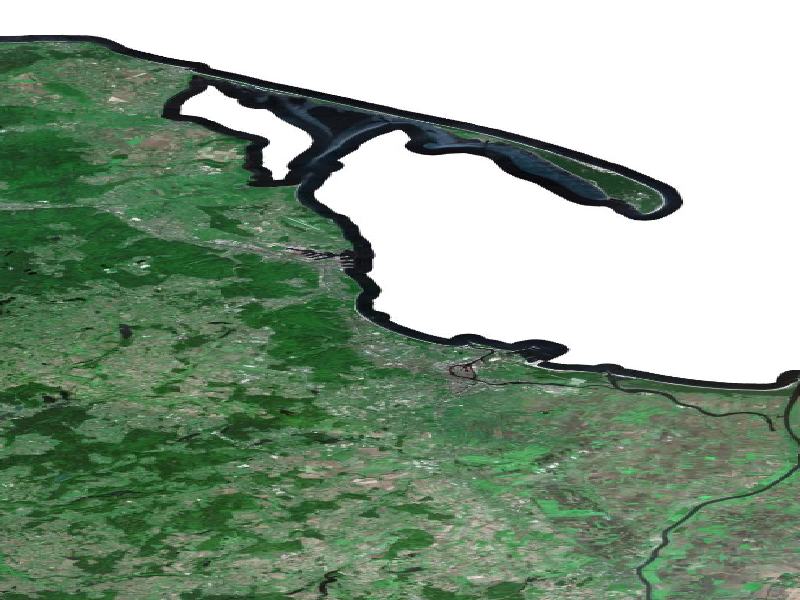
\includegraphics[width=0.7\textwidth]{img/pomorze_gdanskie.png}
    \caption{Pomorze Gdańskie zwrócone przez geoportal}
    \label{fig:pomorze_gdanskie}
\end{figure}

\subsection{WFS}

W ostatnich latach obserwuje się rosące zapotrzebowanie na usługi oparte na danych geograficznych takie jak nawigacja \cite{TRZEBA_COS_ZNALEZC}.
W celu realizacji takich usług, konieczne jest otrzymanie mapy w formacie innym niż rastrowy czy wektorowy, w celu jej dalszego przetworzenia.
Ponadto, w dobie urządzeń mobilnych, możliwość wprowadzania poprawek do danych z dowolnego miejsca wydaje się być koniecznością.
Odpowiedzią na te dwie potrzeby jest standrad Web Feature Service.
Opisuje on, w jaki sposób przesyłać i edytować dane zapisane w metajęzyku GML za pomocą protokołu HTTP.

Metajęzyk Geography Markup Language GML jest sposobem na zapis informacji geograficznych opartym na formacie XML (formalnie rzecz biorąc, jest gramatyką dla XMLa).
Jak każda gramatyka dla XMLa, definiuje plik schematu (XML schema). Są w nim określone następujące typy węzłów:
\begin{itemize}
    \item Feature
    \item Geometry
    \item Coordinate reference system
    \item Topology
    \item Time
    \item Dynamic feature
    \item Coverage (including geographic images)
    \item Unit of measure
    \item Directions
    \item Observations
    \item Map presentation styling rules
\end{itemize}

W ramach typu \textit{geometry}, zdefiniowano 3 rodzaje geometri: punkty, linie łamane oraz wielokaty.
Ponadto, społeczności skupione wokół tych samych projektów często definiują własne typy geometryczne, takie jak drogi.
Przykładowy fragment pliku GML:

\begin{lstlisting}[frame=L, language=xml]
<gml:Point>
    <gml:posList>
        50,100
    </gml:posList>
</gml:Point>
<gml:LineString>
    <gml:posList>
        50,100 100,150
    </gml:posList>
</gml:LineString>
<gml:Polygon>
    <gml:outerBoundaryls>
        <gml:LinearRing>
            <gml:posList>
                10,10 20,10 20,20 10,20 10,10
            </gml:posList>
        </gml:LinearRing>
    </gml:outerBoundaryls>
</gml:Polygon>
\end{lstlisting}

Co więcej, GML dopuszcza także korzystanie z profili. Pozwalają one na uproszczenie tworzenia plików GML. Aby z nich skorzystać, należy je zaimportować \cite{OpeGIS_GML2007}.
Istnieje także język KML, który jest propozycją uproszczenia GMLa. Jest wykorzystywany w usługach geograficznych firmy Google \cite{kulawiak2014}.

Jak wspomniano wyżej, sposób pobierania i edytowania plików GML opisuje standard WFS. Definiuje on zestaw rządań, na które musi odpowiedzieć serwer.
Rządania te mogą być przesyłane za pomocą przeglądarki internetowej. Ponadto, standard dopuszcza używanie zapytań (query). Pozwalają one
na filtrowanie danych dostępnych na serwerze, a następnie na takim podzbiorze danych wykonanie jednego ze zdefiniowanych zapytań \cite{OpenGIS_WFS2010}.
Lista rządań prezentuje się następująco:
\begin{itemize}
    \item GetCapabilities - zwraca informacje opisujące serwer (m.in. jego zawartość);
    \item DescribeFeatureType - zwraca informacje o schematach opisujące niestandarddowe typy (np: drogi) dostępnych na danym serwerze;
    \item GetPropertyValue - informację o wartości konkretnego pola we wszystkich obiektach uzyskanych za pomocą zapytania;
    \item GetFeature - zwraca obiekty na podstawie zapytania;
    \item LockFeature - pozwala na zablokowanie dostępu do zbioru obiektów. Działa podobnie do mechanizmu blokowania znanego z relacyjnych
        baz danych.
    \item GetFeatureWithLock - podobnie jak GetFeature, lecz poza zwróceniem obiektów powienien je również zablokować;
    \item Transaction - służy do tworzenie, zmieniania, zastępowania i usuwania obiektów z serwera;
    \item CreateStoredQuery - zapisuje nowe zapytanie na serwerze;
    \item DropStoredQuery - usuwa zapytanie z serwera;
    \item ListStoredQueries - wypisuje zapytania zapisane na serwerze;
    \item DescribeStoredQueries - zwraca metadane dotyczące wszystkich zapytań zapisanych na serwerze.
\end{itemize}

Przykładowe zapytanie i odpowiedź serwera:
\begin{lstlisting}[frame=L, language=XML]
<!-- Zapytanie -->
<?xml version="1.0" ?>
<GetFeature
    version="2.0.0"
    service="WFS"
    xmlns="http://www.opengis.net/wfs/2.0"
    xmlns:fes="http://www.opengis.net/fes/2.0"
    xmlns:myns="http://www.someserver.com/myns"
    xmlns:xsi="http://www.w3.org/2001/XMLSchema-instance"
    xsi:schemaLocation="http://schemas.opengis.net/wfs/2.0.0/wfs.xsd">
    <Query typeNames="myns:InWaterA_1M">
    <wfs:PropertyName>myns:wkbGeom</wfs:PropertyName>
    <wfs:PropertyName>myns:tileId</wfs:PropertyName>
    <fes:Filter>
        <fes:ResourceId rid="InWaterA_1M.1013"/>
        <fes:ResourceId rid="InWaterA_1M.1014"/>
        <fes:ResourceId rid="InWaterA_1M.1015"/>
    </fes:Filter>
    </Query>
</GetFeature>

<!-- Odpowiedź (fragment) -->

<wfs:member>
    <InWaterA_1M gml:id="InWaterA_1M.1014">
        <wkbGeom>
            <gml:Polygon srsName="urn:ogc:def:crs:EPSG::4326" gml:id="P2">
                <gml:exterior>
                    <gml:LinearRing>
                        <gml:posList>
                        -30.92013931274414 117.6552810668945 -30.92383384704589
                        117.661361694336 -30.93005561828613 117.6666412353516
                        -30.93280601501464 117.6663589477539 -30.93186187744141
                        117.6594467163086 -30.93780517578125 117.6541137695312
                        -30.94397163391114 117.6519470214844 -30.94255638122559
                        117.6455535888672 -30.93402862548828 117.6336364746094
                        -30.92874908447266 117.6355285644531 -30.92138862609864
                        117.6326370239258 -30.92236137390137 117.6395568847656
                        -30.91708374023438 117.6433029174805 -30.91711044311523
                        117.6454467773437 -30.92061042785645 117.6484985351563
                        -30.92061042785645 117.6504135131836 -30.91638946533203
                        117.6504440307617 -30.92013931274414 117.6552810668945
                        </gml:posList>
                    </gml:LinearRing>
                </gml:exterior>
            </gml:Polygon>
        </wkbGeom>
        <id>28021</id>
        <tileId>177</tileId>
    </InWaterA_1M>
</wfs:member> 
\end{lstlisting}

\subsection{WCS}

Dzięki usługom opartym o standrady WMS i WFS możliwe jest przeglądanie, przetwarzanie i edytowanie danych geograficznych.
Rozwój algorytmów służących do przetwarzania danych geograficznych (patrz rozdział 2), powoduje powstawanie dużej ilości danych w postaci pokryć macierzowych
(z ang. \textit{coverages}). Zwykle są to zdjęcia lotnicze i satelitarne, ale mogą też być to chmury punktów czy też numeryczne modele terenu \cite{sudra2012}.
Aby umożliwić dostęp do tego typu informacji, stworzono standrad Web Coverage Service WCS.

W porównaniu do WMS, który przedstawia dane w postaci statycznych map (obrazków), WCS zwraca dane razem z ich opisem oraz semantyką.
Pozwala to na analizowanie, ekstrapolowanie itp. danych, a nie tylko ich wyświetalnie.
W przeciweństwie do WFS, który zwraca dyskretne dane dotyczące zjawisk geograficznych, WFC przedstawia dane w sposób ciągły.
Serwery WCS mogą dostarczać dane w różnych formatach, w szczególności DTED, GeoTIFF, NTF, HDF-EOS i GML. Podobnie jak standard WMS,
WCS także definiuje 3 zapytania \cite{OpenGIS_WCS2012}:
\begin{itemize}
    \item GetCapabilities - zwraca informacje opisujące serwer (m.in. jego zawartość);
    \item DescribeCoverage - zwraca listę wszystkich dostępnych pokryć macierzowych wraz z ich opisami;
    \item GetCoverage - zwraca rządane pokrycie macierzowe.
\end{itemize}

\section{GeoServer i MapServer}

Istnieją różne technologie dostępu do danych geograficznych, jak chociażby opisane w \autoref{chap:protokoly} standardy WMS, WFS i WCS.
Jednakże są to tylko standardy. Konieczne jest stworzenie oprogramowania, które będzie je implementowało, a tym samym umożliwi
uzytkownikom dostęp do danych. GeoServer oraz MapServer są przykładami takiego oprogramowania.

GeoServer jest serwerem pozwalającym na pozyskiwanie i edytowanie danych geograficznych.
Jest napisany w języku Java jako oprogramowanie typu open-source.
Jako tego typu projekt, jest tworzony, testowany i rozwijany przez grupę osób i organizacji rozsianych po całym świecie.
GeoServer stanowi referencyjną implementację standardów WFS i WCS. Ponadto posiada certyfikat wysokiej wydajności implementacji WMSa.
Serwer ten obsługuje dane geograficzne różnych rodzajów, w tym formaty bazodanowe (PostGIS, Oracle Spatial) jak i plikowe (Shapefiles, GeoTIFF)
jako źródła danych. Poza tym możliwe jest też wykorzystanie innego serwera WMS czy WFS jako źródła.
Format danych zwracanych zależny jest od wykorzystywanego protokołu. Dodatkowo, wraz z serwerem dostarczana jest wbudawana aplikacja
oparta na OpenLayers (\ref{chap:OpenLayers}), która umożliwia podgląd umieszczanych map bez konieczności poznawania składni zapytań \cite{GeoServerManual2016}.

GeoServer nie istnieje w próżni. Do jego działania konieczna jest baza danych (w tym przypadku PostGIS). Dodatkowo istnieje też usługa
GeoWebCache, która zapisuje odpowiedzi na zapytania. Przyspiesza to działanie serwera z punktu widzenia użytkownika, który nie musi
czekać na wygenerowanie odpowiedzi \cite{OpenGeo2012}. Na rysunku \ref{fig:GeoServerArchitecture} przedstawiono tę architekturę, wraz z zaznaczoną
aplikacją użytkownika.

\begin{figure}[h!]
    \centering
    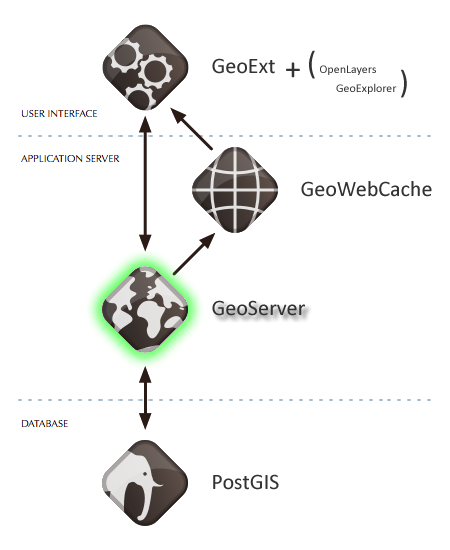
\includegraphics[width=0.4\textwidth]{img/geoserver_architecture.png}
    \caption{Architektura GeoServer}
    \source{http://presentations.opengeo.org/2012\_FOSSGIS/suiteintro/\_images/stack\_geoserver.png}
    \label{fig:GeoServerArchitecture}
\end{figure}

Jak wspomniano wyżej, GeoServer obsługuje wiele różnych standardów OGC, w tym WMS. W momencie przyjścia rządania o dostarczenie mapy,
serwer wykonuje następujące operacje:
\begin{enumerate}
    \item Ładowanie danych z bazy (opcjonalne filtrowanie)
    \item Nałożenie stylu
    \item Renderowanie obrazka i zwrócenie do użytkownika
\end{enumerate}
Na rysunku \ref{fig:geoserver_WMS_architecture} przedstawiono jak przebiega ten proces.

\begin{figure}[h!]
    \centering
    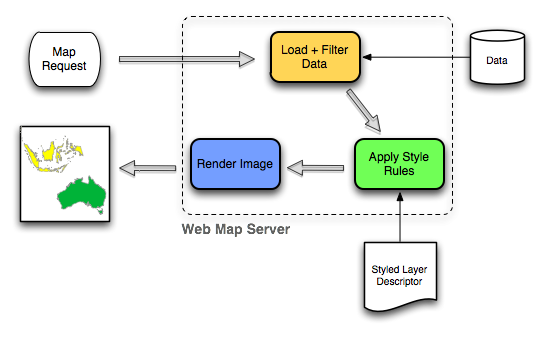
\includegraphics[width=0.7\textwidth]{img/geoserver_wms_architecture.png}
    \caption{Schemat odpowiedzi GeoServera na zapytanie GetMap}
    \source{http://presentations.opengeo.org/2012\_FOSSGIS/suiteintro/\_images/wms.png}
    \label{fig:geoserver_WMS_architecture}
\end{figure}

Obsługa GeoServera możliwa jest z poziomu przeglądarki. Nie ma konieczności edytowania plików konfiguracyjnych
w celu dodania nowego źródła danych, utworzenia nowej warstwy czy zdefiniowania nowego stylu. Dzięki temu rozwiązaniu
GeoServer może być łatwo wykorzystywany także przez użytkowników nie zaznajomionych z obsługą typowych aplikacji serwerowych.
Na rysunku \ref{} przedstawiono interfejs WWW dostarczany przez GeoServer.

MapServer stanowi alternatywę dla GeoServera. Podobnie jak poprzednik, MapServer stanowi implementację różnych standardów,
w tym WMS, WFS i WCS. Jest napisany w języku C/C++. Rozwijany jest przez wiele firm z całego świata jako projekt open-source.
Podstawowoym źródłem danych dla MapServera są pliki shapefile, ale możliwe jest też wykorzystanie innych źródeł. 
Moożliwe jest też wykorzystanie innego serwera WMS czy WFS jako źródła danych \cite{MapServer2011}.
Format danych zwracanych jest zależny od wybranego protokołu.

Najprostsza aplikacja oparta o MapServer składa się z następujących komponentów:
\begin{itemize}
    \item Dane wejściowe - mogące pochodzić z loklanych baz danych, jak i zewnętrznych serwerów;
    \item Aplikacje MapServer i MapScript - odpowiedzialne za obsługe rządania. Ich konfiguracja zawarta jest w plikach Mapfile
    \item Serwer WWW (Apache) - odpowiada za komunikację poprzez protokół HTTP z klientem
\end{itemize}

Architektura ta została przedstawiona na rysunku \ref{fig:mapserver_architecture}.
\begin{figure}[h!]
    \centering
    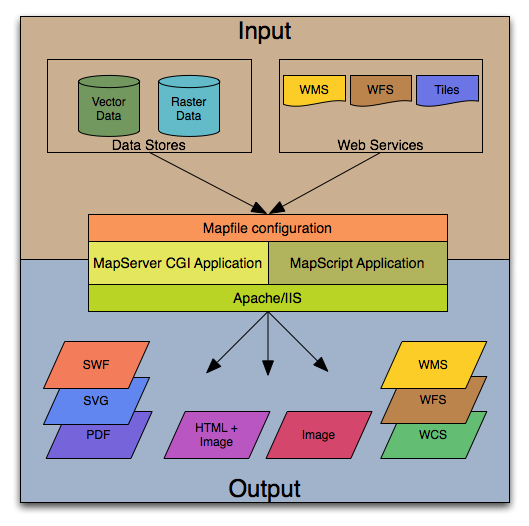
\includegraphics[width=0.7\textwidth]{img/mapserver_architecture.png}
    \caption{Architektura MapServera}
    \source{http://mapserver.org/\_images/architecture.png}
    \label{fig:mapserver_architecture}
\end{figure}

W przeciwieństwie do GeoServera, MapServer nie posiada interfejsu graficznego. Wszystkie operacje takie jak,
dodanie nowej mapy, zmiana stylu czy dodanie nowej warstwy, muszą być być przeprowadzane przy użyciu plików
konfiguracyjnych typu Mapfile (.map). Są to pliki tektowe, których konwencja przypomina tą znaną z plików
konfiguracyjnych dla serwisów działających w systemach linux. W ramach pliku mapfile można zdefiniować następujące
obiekty \cite{MapServer2011}:
\begin{itemize}
    \item MAP - obiekt odzwierciedlający całą mapę;
    \item LAYER - obiekt odzwierciedlający warstwę mapy. Musi być typu \textit{RASTER}, wtedy warstwa bedzie warstwą rastrową,
        bądź typu \textit{POINT, LINE} lub \textit{POLYGON} - wtedy warstwa będzie warstwą wektorową;
    \item CLASS - obiekt przechowujący dane dotyczące styli;
    \item SYMBOL - symbol do umieszczenia na mapie;
    \item LABEL - umożliwia dodanie napisu na mapie.
\end{itemize}

Poniżej przedstawiono przykładowy plik konfiguracyjny wraz ze zwróconą mapą (rysunek \ref{fig:mapserver_config}).

\begin{lstlisting}[frame=L]
MAP
    NAME "sample"
    STATUS ON
    SIZE 600 400
    SYMBOLSET "../etc/symbols.txt"
    EXTENT -180 -90 180 90
    UNITS DD
    SHAPEPATH "../data"
    IMAGECOLOR 255 255 255
    FONTSET "../etc/fonts.txt"

    #
    # Start of web interface definition
    #
    WEB
        IMAGEPATH "/ms4w/tmp/ms_tmp/"
        IMAGEURL "/ms_tmp/"
    END # WEB

    #
    # Start of layer definitions
    #
    LAYER
        NAME 'global-raster'
        TYPE RASTER
        STATUS DEFAULT
        DATA bluemarble.gif
    END # LAYER
END # MAP
\end{lstlisting}

\begin{figure}[h!]
    \centering
    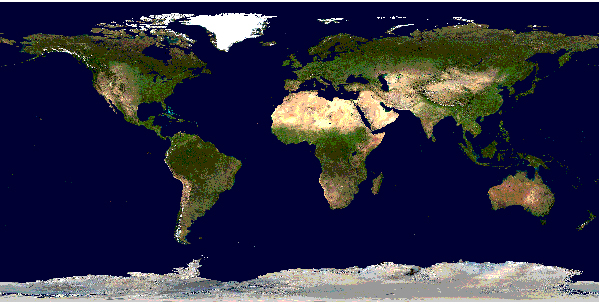
\includegraphics[width=0.7\textwidth]{img/mapserver_config.jpg}
    \caption{Przykładowa odpowiedź od MapServera}
    \source{http://mapserver.org/\_images/bluemarble-rendered.jpg}
    \label{fig:mapserver_config}
\end{figure}

\section{OpenLayers i Leaflet.js}
\label{chap:OpenLayers}

W poprzednim rozdziale opisano dwa konkurencyjne rozwiązania serwerowe, które, ogólnie rzecz ujmując, służą do dostarczania danych geograficznych użytkownikowi.
Do komunikacji z takim serwerem, konieczne jest posiadanie odpowiedniego klienta. Zgodnie ze standardami OCG \cite{OpenGIS_WMS2006,OpenGIS_WFS2010,OpenGIS_WCS2012}
komunikacja możliwa jest przy użyciu przeglądarki internetowej. Jednakże, ręczne tworzenie zapytań jest długotrwałe i mało wygodne. Dlatego powstały biblioteki
dla języka JavaScript, ułatwiające komunikację z serwerami WMS, WFS i WCS. W tym podrozdziale zostaną opisane dwie z nich - OpenLayers i Leaflet.js

OpenLayers powstało w 2006 roku jako odpowiedź na pojawienie się zamkniętych Google maps.
Za cel postawiono umożliwienie użytkownikom wyświetlania na swoich stronach map w sposób podobny do tego, znanego z usług Google.
Jednakże projekt miał umożliwiać tworzenie map z dowolnego źródła i miał być open-sourcowy \cite{website:OpenLayersHistory}.
Akutalnie rozwiajana jest wersja 3 biblioteki, pomimo że sporo aplikacji ciągle używa poprzedniej wersji.

Aplikacja wykorzystująca OpenLayers może korzystać ze źródeł w wielu formatach. Należą do nich:
\begin{itemize}
    \item Źródła dostarczające dane w formacie kafelkowym np: OSM, Bing;
    \item Dane wektorowe w formatach GeoJSON, TopoJSON, KML i GML;
    \item Dane dostarczane przez serwer zgodny ze standardami OGC.
\end{itemize}

Aplikacje korzystające z OpenLayers wykorzystują pewne standardowe komponenty dostarczane przez bibliotekę. Podstawowym jest mapa (\textit{ol.map}).
Jest ona rysowana w obiekcie celu (\textit{target}). Parametry obiektu mapy mogą być określane przy jej inicjalizacji lub po jej utworzeniu.
Obiekt mapy nie jest odpowiedzialny za oddalanie, przybliżanie czy przesuwanie mapy. Do tego celu służy obiekt widoku(\textit{ol.View}).
Dodatkwo należy zdefiniować źródło danych (\textit{ol.source.Source}). 
Aby wyświetlić dane ze źródła, potrzebny jest obiekt warstwy (\textit{ol.layer}). Aktualnie istnieją 3 rodzaje warstw:
\begin{itemize}
    \item \textit{ol.layer.Tile} - rodzaj warstwy dla danych w postaci gotowych kafelków;
    \item \textit{ol.layer.Image} - rodzaj warstwy do wyświetlania obrazków;
    \item \textit{ol.layer.Vector} - rodzaj warstwy do wyświetlania danych wektorowych.
\end{itemize}

Oczywiście, na jednej mapie może być dowolnie wiele warstw. Wykorzystując opisane komponenty można stworzyć taką przykładową aplikację:

\begin{lstlisting}[frame=L, language=JavaScript]
<div id="map" style="width: 100\%,height:400px"></div>
<script>
  new ol.Map({
    layers: [
      new ol.layer.Tile({source: new ol.source.OSM()})
    ],
    view: new ol.View({
      center: [0, 0],
      zoom: 2
    }),
    target: 'map'
  });
</script>
\end{lstlisting}

Wynik działania tej aplikacji przedstawiono na rysunku \ref{fig:openlayers_example}.

\begin{figure}[h!]
    \centering
    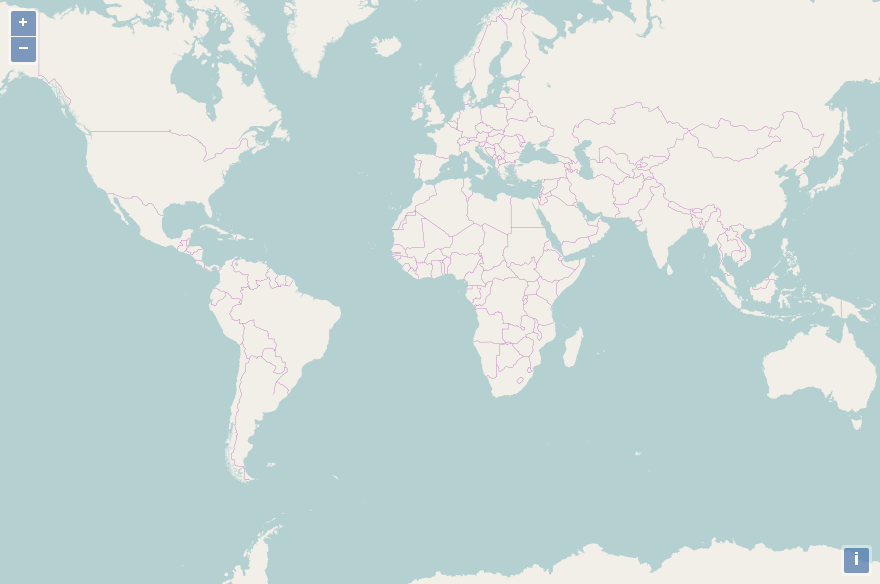
\includegraphics[width=1.0\textwidth]{img/openlayers_example.png}
    \caption{Przykładowa aplikacja OpenLayers}
    \source{własne}
    \label{fig:openlayers_example}
\end{figure}


\chapter{Implementacja algorytmu}
\label{chap:implementacja}

Dane pochodzące ze skanowania laserowego wysokiej rozdzielczości zajmują bardzo dużo miejsca, przez co
dostęp do nich poprzez Internet wymaga relatywnie długiego czasu (rzędu kilkunastu sekund). Powoduje to,
iż niemożliwym jest zbudowanie systemu który w czasie rzeczywistym przedstawiałby te dane w sposób podobny
do aktualnie dostępnych w Internecie map, jak Google Maps. Aby zaradzić temu problemowi, stworzono dwa algorytmy.
Ich celem było takie przetworzenie danych wejsciowych, aby zmiejszyć ich objętość jednoczesnie nie tracąc zawartych w nich informacji.
W niniejszym rozdziale znajdują się opisy tych algorytmów oraz opis przekształcania ich do formatu shapefile w celu udostępnienia
poprzez GeoServer.

\section{Algorytm Naiwny}

W celu szybkiego otrzymania wyników zdecydowano się na stworzenie prostego (naiwnego) algorytmu. Opierał się on na następujących założeniach:
\begin{itemize}
    \item Dane wejściowe posiadają wysoką rozdzielczość (rzędu kilkudziesieciu punktów na metr)
    \item Punkty znajdujące się blisko siebie (tzn. odległość $d$ ze wzoru \ref{eq:odleglosc_euklidesowa} mniejsza niż stała $C$), są fragmentem tej samej powierzchni
\end{itemize}

\noindent Algorytm ten składa się z następujących faz:
\begin{enumerate}
    \item Wczytywanie danych
    \item Wstępne sortowanie
    \item Przypisywanie do zbiorów
    \item Filtracja zbiorów
    \item Znalezienie otoczki wklęsłej dla każdego ze zbiorów
\end{enumerate}

\subsection{Wczytywanie danych}

Dzięki wykorzystaniu biblioteki liblas \cite{website:libLASPython}, odczytywanie danych z plików w formacie .las jest niezwykle proste.
Całość ogranicza się do zaimportowania odpowiedniej klasy i wykorzystania prostej pętli for, jak przedstawiono
w algorytmie \ref{lis:wczytanie_danych}

\begin{lstlisting}[frame=L, language=python, caption={Wczytywanie danych}, label={lis:wczytanie_danych}]
from liblas import file

def read_from_file(name):
    points = []
    f = file.File(name)
    for p in f:
        points.append(MyPoint(p.x, p.y, p.z, classification=p.classification))
    f.close()

    return points
\end{lstlisting}

Punkty są przechowywane w pamięci jako obiekty klasy \textit{MyPoint}. W ramach takiego obiektu przechowywane są informacje dotyczące
współrzędnych punktu, przynależności do zbioru oraz klasyfikacji. Obiekt może też określić swoją odległość od innego punktu
za pomocą metody \textit{get\_distance} oraz określić czy dany punkt jest jego sąsiadem przy użyciu metody \textit{is\_neighbour}.

\subsection{Wstępne sortowanie}
\label{chap:wstepne_sortowanie}

Jak stwierdzono we wstępie, jednym z założeń jest, iż punkty znajdujące się blisko siebie są fragmentem tej samej powierzchni.
Oznacza to konieczność porównywania ze sobą punktów w systemie każdy z każdym, aby stwierdzić, które z nich należą do tego samego zbioru.
Jedakże takie podejście oznacza złożoność obliczeniową rzędu $O(N^2)$, która,  przy ilości punktów wynoszącą kilka milionów, jest niedopuszczalna.
Aby przyspieszyć obliczenia, zdecydowano się na wstępne posortowanie punktów, aby możliwe było porównywanie danego punktu tylko z punktami z 
jego najbliższego otoczenia.

Sortowanie polega na umieszczeniu punktów w macierzy $[M x N]$, której wymiary odpowiadają różnicy między największa i najmniejszą wartością
współrzędnych $x, y$ punktu $p$ ze zbioru punktów wejściowych $P$:
\begin{eqnarray}
    M = max(p.x) - min(p.x) \bigvee p \in P \\
    N = max(p.y) - min(p.y) \bigvee p \in P
\end{eqnarray}

\noindent Punkty umieszczane są w odpowiadjącym ich współrzędnym komórkach macierzy (algorytm \ref{lis:sortowanie_punktow}).

\begin{lstlisting}[frame=L, language=python, caption={Sortowanie punktów}, label={lis:sortowanie_punktow}]
sorted_points = [[ [] for _ in range(0, N)] for _ in range(0, M)]

for p in P:
    x = int(math.floor(p.x - xmin))
    y = int(math.floor(p.y - ymin))
    sorted_points[x][y].append(p)

\end{lstlisting}

W uproszczeniu można powiedzieć, iż algorytm ten powoduje nałożenie siatki na chmurę punktów, co zostało zobrazowane na rysunku \ref{fig:sortowanie_punktow}

\begin{figure}[h!]
	\centering
    \begin{subfigure}[b]{0.3\textwidth}
        \includegraphics[width=\linewidth]{img/sortowanie_punktow1.png}
    \end{subfigure}%
	\quad
    \begin{subfigure}[b]{0.3\textwidth}
        \includegraphics[width=\linewidth]{img/sortowanie_punktow2.png}
    \end{subfigure}%
    \caption{Sortowanie punktów w zbiorze}
    \label{fig:sortowanie_punktow}
\end{figure}

\subsection{Przypisywanie do zbiorów}
W tym etapie następuje podział punktów na podzbiory na podstawie sąsiedztwa. Punkty znajdujące się blisko siebie,
są zaliczane do jednego zbioru i tym samym traktowane jako fragmenty tej samej powierzchni. Dzięki posortowaniu
możliwe jest porównywanie tylko punktów leżących blisko siebie w projekcji dwuwymiarowej (z pominięciem składowej $z$).
Algorytm wygląda następująco:

\begin{lstlisting}[frame=L, language=python, caption={Podział punktów na zbiory w algorytmie naiwnym}, label={lis:podzial_naiwny}]
def find_neighbour(point, neighbour_points, sets):
    if point.point_set is None:
        point.point_set = len(sets)
        sets.append([point])
    for p in neighbour_points:
        if point.is_neighbour(p):
            if p.point_set is None:
                sets[point.point_set].append(p)
                p.point_set = point.point_set
            elif point.point_set != p.point_set:
                union_sets(point.point_set, p.point_set, sets)
\end{lstlisting}

W funkcji przedstawionej na listingu \ref{lis:podzial_naiwny} dokonuje się całe clou algorytmu naiwnego.
W pierwszej części (linie 2-4) aktualnie badany punkt (\textit{point}) tworzy nowy jednoelementowy zbiór,
jeśli nie należy do żadnego.

Następnie punkt ten jest porównywany ze wszystkimi pobliskimi\footnote{pobliskie punkty to takie,
które znajdują się w tej samej lub sąsiedniej komórce macierzy. Patrz \autoref{chap:wstepne_sortowanie}}
punktami. Najpierw sprawdzana jest, czy dwa punkty są sąsiadami tzn. czy leżą na tej samej powierzchni. 
Określa się to poprzez obliczenie odległości $d$ między nimi. Odległość ta jest określana przez metrykę euklidesową:
\begin{equation} \label{eq:odleglosc_euklidesowa_ogolna}
    d(A,B) = \sqrt{\sum\limits_{i=1}^n((x_{iA}-x_{iB})^2)}
\end{equation}

\noindent Gdzie $n$ określa liczbę wymiarów. Dla przypadku trójwymiarowego, równanie \ref{eq:odleglosc_euklidesowa_ogolna} można uprościć do:
\begin{equation} \label{eq:odleglosc_euklidesowa}
    d(A,B) = \sqrt{(x_A - x_B)^2 + (y_A - y_B)^2 + (z_A - z_B)^2}
\end{equation}

Gdzie $x, y, z$ są kolejnymi współrzędymi punktu. Po obliczeniu odległości $d$ na podstawie równania \ref{eq:odleglosc_euklidesowa}
jest sprawdzane, czy jest ona mniejsza niż stała $C$\footnote{Dodatkowo bierze się pod uwagę, czy punkty są tak samo sklasyfikowane.
Jeśli tak, to wtedy $C = C*2$.}. Jeżeli tak, uznaje się że punkty są sąsiadami. Cały proces został zilustrowany na
rysunku \ref{fig:sprawdzanie_sasiedztwa}

\begin{figure}[h!]
    \centering
    \begin{subfigure}[b]{0.3\textwidth}
        \includegraphics[width=\linewidth]{img/sasiedztwo_punktow1.png}
        \caption {punkty należą do tego samego zbioru (d < C)}
    \end{subfigure}
    \quad
    \begin{subfigure}[b]{0.3\textwidth}
        \includegraphics[width=\linewidth]{img/sasiedztwo_punktow2.png}
        \caption {punkty nie należą do tego samego zbioru (d > C)}
    \end{subfigure}%
    \caption{Sprawdzanie sąsiedztwa punktów wobec punktu A}
    \label{fig:sprawdzanie_sasiedztwa}
\end{figure}


Po sprawdzeniu sąsiedztwa, jeżeli drugi z punktów nie należy do żadnego zbioru, przypisuje się go do tego samego zbioru, co badany punkt \textit{point}.
W przeciwnym przypadku (gdy oba punkty należą do różnych zbiorów), zbiory te są łączone przy wykorzystaniu metody \textit{union\_set}.
Metoda ta przepisuje wszystkie punkty z mniejszego zbioru do większego (dbając przy tym o poprawność indeksów).

\subsection{Filtracja zbiorów}

Na tym etapie zostają odrzucone zbiory puste (mogły powstać wskutek łączenia zbiorów) oraz zbiory zawierające
mniej niż $F$ punktów. Pozwala to odrzucić bardzo małe zbiory, które można zaniedbać przy odpowiednim
poziomie szczegółowości.

\subsection{Znalezienie otoczki wklęsłej dla każdego ze zbiorów}
\label{chap:upraszczanie}

Otoczką wklęsła zbioru punktów na płaszczyźnie nazywamy najmniejszy wielokąt taki, że wszystkie punkty z tego
zbioru leżą albo wewnątrz tego wielokąta, albo na jego krawędziach. Znalezienie tego wielokąta będzie polegało na
stworzeniu najpierw otoczki wypukłej dla zadanego zbioru (przy pomocy triangulacji Delaunaya), a następnie takiego
odfiltrowania krawędzi, aby stworzyć przybliżenie otoczki wklęsłej.

Otoczką wypukłą zbioru punktów na płaszczyźnie nazywamy najmniejszy wielokąt wypukły taki, że wszystkie punkty z tego
zbioru leżą albo wewnątrz tego wielokąta, albo na jego krawędziach \cite{website:OtoczkaTriangulacja}.
Triangulacja Delaunaya jest podziałem otoczki wypukłej na trójkąty. W związku z tym, problem znalezienia otoczki
można sprowadzić do problemu tworzenia triangulacji.

W ramach algorytmu szukamy otoczki zbioru punktów rzutowanych na powierzchnię dwuwymiarową.
Zakładamy, iż każdy znaleziony zbiór jest reprezentacją jakiejś powierzchni płaskiej,
w związku z tym po znalezieniu otoczki, można odrzucić wszystkie punkty znajdujące się wewnątrz.
Będą one interpolowane poprzez punkty graniczne.
Odrzucenie większości punktów skutkuje zmniejszeniem ilości pamięci koniecznej do przechowywania informacji. Jednocześnie autor ma
świadomość ograniczeń tego rozwiązania (wywołanych przez rzutowanie), jak np: upraszczanie ostrosłópów do płaskich powierzchni, co przedstawiono
na rysunku \ref{fig:upraszczanie_otoczki}.

\begin{figure}[h!]
    \centering
    \begin{subfigure}[b]{0.3\textwidth}
        \includegraphics[width=\linewidth]{img/upraszczanie_otoczki1.png}
        \caption {Oryginalne dane}
    \end{subfigure}
    \quad
    \begin{subfigure}[b]{0.3\textwidth}
        \includegraphics[width=\linewidth]{img/upraszczanie_otoczki2.png}
        \caption {Dane po zrzutowaniu}
    \end{subfigure}%
    \caption{Rzutowanie na powierzchnię dwuwymiarową powoduje utracenie części informacji}
    \label{fig:upraszczanie_otoczki}
\end{figure}

Wykorzystanie triangluacji Delaunaya nie jest skomplikowane. Algorytm obliczający triangluacje
dla zbioru punktów jest dostępny jako część pakietu \textit{scipy}. Dodatkowo wykorzystano pakiet \textit{shapely},
który ułatwił zarządzanie figurami geometrycznymi. Cały algorytm (wykorzystujący wspomniane pakiety)
prezentuje się następująco:

\begin{lstlisting}
# Źródło: http://blog.thehumangeo.com/2014/05/12/drawing-boundaries-in-python/
def alpha_shape(points, alpha):
   def add_edge(edges, edge_points, coords, i, j):
        """
        Add a line between the i-th and j-th points,
        if not in the list already
        """
            if (i, j) in edges or (j, i) in edges:
                # already added
                return
            edges.add( (i, j) )
            edge_points.append(coords[ [i, j] ])

    coords = np.array([point.x, point.y
                       for point in points])
    tri = Delaunay(coords)
    edges = set()
    edge_points = []
    # loop over triangles:
    # ia, ib, ic = indices of corner points of the
    # triangle
    for ia, ib, ic in tri.vertices:
        pa = coords[ia]
        pb = coords[ib]
        pc = coords[ic]
        # Lengths of sides of triangle
        a = math.sqrt((pa[0]-pb[0])**2 + (pa[1]-pb[1])**2)
        b = math.sqrt((pb[0]-pc[0])**2 + (pb[1]-pc[1])**2)
        c = math.sqrt((pc[0]-pa[0])**2 + (pc[1]-pa[1])**2)
        # Semiperimeter of triangle
        s = (a + b + c)/2.0
        # Area of triangle by Heron's formula
        area = math.sqrt(s*(s-a)*(s-b)*(s-c))
        circum_r = a*b*c/(4.0*area)
        # Here's the radius filter.
        #print circum_r
        if circum_r < 1.0/alpha:
            add_edge(edges, edge_points, coords, ia, ib)
            add_edge(edges, edge_points, coords, ib, ic)
            add_edge(edges, edge_points, coords, ic, ia)
    m = geometry.MultiLineString(edge_points)
    triangles = list(polygonize(m))
    return cascaded_union(triangles), edge_points 
\end{lstlisting}

Pierwszym etapem tworzenia otoczki wypukłej jest zrzutowanie danych na powierzchnię dwuwymiarową (linie 14-15).
Następnie zostaje utworzona triangulaja Delaunay. Potem następuje przejście po wszystkich trójkątach nowo
utworzonej siatki i dla każdego z nich policzenie promienia okręgu opisanego na tym trójkącie (linie 22-34). Dzięki
parametrowi \textit{alpha} możliwe jest odrzucenie części trójkątów (tych, dla których promień okręgu opisanego jest większy niż $1/alhpa$).
Powoduje to, że otoczka z wypukłej staje się wklęsłą - bardziej odpowiada kształtowi rzeczywistych obiektów.
Ostatnim etapem jest utworzenie obiektu typu \textit{shapely.geometry.polygon.Polygon}. Obiekt ten posiada w sobie informację
o punktach granicznych, tworzących otoczenie. Przykładowe efekty działania funkcji \textit{alpha\_shape} dla różnych wartości 
parametru \textit{alpha} przedstawiono na rysunku \ref{fig:triangulacja_alpha}.

\begin{figure}[h!]
    \centering
    \begin{subfigure}[b]{0.33\textwidth}
        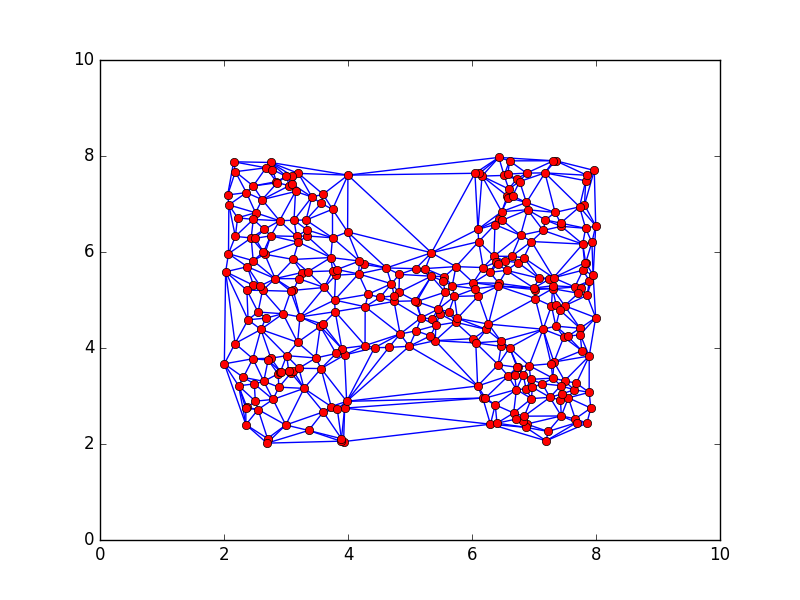
\includegraphics[width=\linewidth]{img/triangulacja1.png}
        \caption {alpha = 0.4}
    \end{subfigure}
    \begin{subfigure}[b]{0.33\textwidth}
        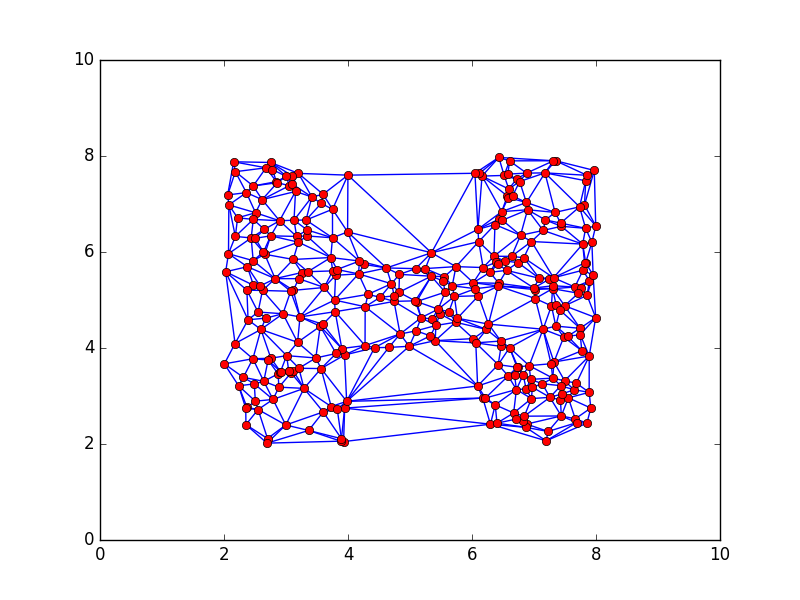
\includegraphics[width=\linewidth]{img/triangulacja2.png}
        \caption {alpha = 0.8}
    \end{subfigure}%
	\begin{subfigure}[b]{0.33\textwidth}
		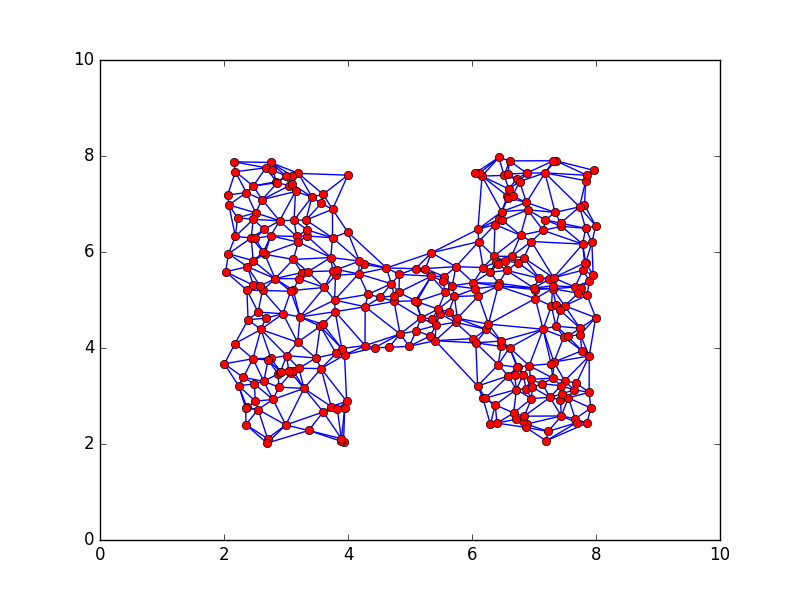
\includegraphics[width=\linewidth]{img/triangulacja3.png}
		\caption {alpha = 1.6}
	\end{subfigure}
    \caption{Efekty metody alpha\_shape przy różnych współczynnikach alpha}
    \label{fig:triangulacja_alpha}
\end{figure}

\section{Algorytm iteracyjny}

Algorytm naiwny dał nadspodziewanie dobre wyniki (\autoref{chap:wyniki}), jednakże posiada jedną wadę:
ciężko poprawić jakość wyników. W związku z tym pojawiła się idea, aby stworzyć nowy algorytm, częściowo
opierając się na poprzednim. W stosunku do algorytmu naiwnego poczyniono następujące zmiany:
\begin{itemize}
    \item Algorytm ma w sposób iteracyjny poprawiać dokładność wyników
    \item Algorytm ma brać pod uwagę też inne czynniki niż odległość punktów od siebie
\end{itemize}

\noindent Kolejne kroki algorytmu pozostały takie same, dla przypomnienia:
\begin{enumerate}
    \item Wczytywanie danych
    \item Wstępne sortowanie
    \item Przypisywanie do zbiorów
    \item Filtracja zbiorów
    \item Znalezienie otoczki wklęsłej dla każdego ze zbiorów
\end{enumerate}

Zmieniony został sposób przypisywania do zbiorów. Na początku wyszukiwane są wszystkie zbiory będące w pobliżu badanego punktu.
Jeżeli nie znaleziono żadnego, tworzy się nowy zbiór zawierający tylko badany punkt.
Jeśli znaleziono jeden zbiór, przypisywano badany punkt do niego.
W syutuacji kiedy znaleziono więcej niż jeden zbiór następuje ważenie. Bierze ono pod uwagę odległość punktu od najbliższego
punktu należącego do zbioru oraz różnicę między średnią wysokością punktów w zbiorze a wysokością badanego punktu podzieloną
przez odchylenie standardowe tego zbioru. Algorytm został przedstawiony na rysunku \ref{fig:algorytm_iteracyjny}. W listingu
\ref{lis:wazenie} przedstawiono jak przebiega faza ważenia.

\begin{figure}[h!]
    \centering
    \includegraphics[width=0.6\linewidth]{img/algorytm_iteracyjny.png}
    \caption{Pętla algorytmu iteracyjnego}
    \label{fig:algorytm_iteracyjny}
\end{figure}

\begin{lstlisting}[frame=L, language=python, label={lis:wazenie}, caption={Ważenie punktów w algorytmie iteracyjnym}]
# calculate which set suits best
max_score = 0
for set_dict in neighbour_sets:
    s = set_dict['set']
    if s.sd() > 0:
        score = abs(s.average() - point.z) / s.sd()
    elif s.sd() == 0.0:
        score = abs(s.average() - point.z) / 0.00001
    set_dict['score'] = score
    if score > max_score:
        max_score = score

max_abs_score = 0
target = None
for set_dict in neighbour_sets:
    if max_score:
        set_dict['score'] = (set_dict['score'] / max_score) / 2.0 + set_dict['distance']
    else:
        set_dict['score'] = set_dict['distance']
    set_dict['score'] = 1 - set_dict['score']

    if set_dict['score'] > max_abs_score:
        target = set_dict
        max_abs_score = set_dict['score']

if point.point_set:
    point.point_set.delete_point(point)
point.point_set = target['set']
target['set'].append(point)
\end{lstlisting}

Fazę ważenia można podzielić na dwa etapy. W pierwszym z nich liczone jest o ile odchyleń standardowych
wartość wysokości danego punktu odbiego od średniej ze zbioru (linie 5-6). Wartość ta stanowi wstępną wartość punktową, jakią uzyskał dany zbiór.
Jeżeli dla danego zbioru odchylenie standardowe wynosi 0\footnote{Będzie tak, jeżeli w zbiorze będzie tylko jeden punkt,
lub gdy wszystkie punkty ze zbioru mają taką samą wysokość.},
wtedy na potrzeby obliczeń przyjmuje się iż odchylenie standardowe jest bardzo małą liczbą ($10^{-5}$).

W drugim etapie następuje normalizacja liczby punktów do przedziału $<0; 0,5>$ poprzez podzielenie wartości punktowej
przez maksymalny wynik uzyskany przez jeden ze zbiorów pomnożonej przez 2. Następnie do znormalizowanego wyniku punktowego
dodaje się odległość\footnote{Odległość jest znormalizowana do przedziału $<0; 0,5>$} 
między badanym punktem a najbliższym punktem ze zbioru (linie 16-17).
Jeżeli maksymlna wartośc punktowa uzyskana w poprzednim etapie wynosi 0, wtedy na potrzeby ostatecznej punktacji
bierze się pod uwagę tylko odległość. Ostateczny wynik uzyskuje się odejmując 1 od uprzednio uzyskanego wyniku (linia 20).
Na końcu przypisuje się punkt do zbioru, który uzyskał największą ilość punktów.

\section{Przekształcanie do formatu shapefile}

Po podziale surowych danych na zbiory (będące w istocie wielokątami), konieczne jest
przekształcenie ich do formatu shapefile. Dzięki temu możliwe będzie wyśwetlanie wyników
za pomocą aplikacji implementujących standardy OGC, jak np: GeoServer.

Do kowersji danych wykorzystano pakiet \textit{osgeo}. Jest to pakiet który umożliwia
wykorzystywanie tzw. bilbioteki GDAL (Geospatial Data Abstraction Library). Pozwala ona
na tworzenie i manipulowanie obiektami geograficznymi, takimi jak punkty, linie i wielokąty.
Dodatkowo posiada wsparcie dla wielu różnych projekcji geograficznych. Wykorzystanie tej
biblioteki do konwersji przedstawiono na listingu \ref{lis:konwersja}.

\begin{lstlisting}[frame=L, language=python, caption={Konwersja danych do formatu SHP}, label={lis:konwersja}]
import osgeo.ogr as ogr
import osgeo.osr as osr

spatialReference = osr.SpatialReference()
spatialReference.ImportFromEPSG(2180)

driver = ogr.GetDriverByName('ESRI Shapefile')
shapeData = driver.CreateDataSource('data.shp')

layer = shapeData.CreateLayer('Layer1', spatialReference, ogr.wkbPolygon)

for surface in surface_list:
	ring = ogr.Geometry(ogr.wkbLinearRing)
	for x, y, z in zip(points[0], points[1], points[2]):
	    ring.AddPoint(x, y, z)
	poly = ogr.Geometry(ogr.wkbPolygon)
	poly.AddGeometry(ring)
	result.append(poly)
	
	feature = ogr.Feature(layer.GetLayerDefn())
	feature.SetGeometry(poly)
	layer.CreateFeature(feature)
	feature.Destroy()

shapeData.Destroy()

\end{lstlisting}

Na początku tworzona jest georeferencja w formacie EPSG 2180 (linie 4-5). Jest to georeferencja w której zostały
zebrane wejściowe dane lidar. Następnie tworzony jest sterownik, w tym wypadku do tworzenia plików .SHP, oraz otwierany
jest deskryptor na plik wynikowy (linie 7-8). Potem tworzona jest nowa warstwa, umieszczana we wcześniej zadeklarowanej
georeferencji. Dodatkowo deklarowane jest, iż warstwa ta zawierać będzie wielokąty (linia 10). W pętli for przechodzimy po kolei
przez wszystkie punkty tworzące wszystkie wielokąty i dodajemy je do stworzonej warstwy (linie 12-23). Na końcu niszczony jest
deskryptor na plik, co powoduje zapisanie przetworzonych informacji na dysku (linia 25).

\chapter{Wyniki oraz omówienie}
\label{chap:wyniki}

W celu porównania obu rozwiązań przedstawionych w \autoref{chap:implementacja} przeprowadzono szereg testów.
Oceniono poprawność działania algorytmu na uproszczonych, automatycznie generowanych danych a także na podstawie
rzeczywistych danych pochodzących ze skanowania laserowego. Sprawdzono również czasy przetwarzania dla poszczególnych
algorytmów oraz stwierdzono, czy możliwe jest wykorzystanie obu algorytmów jednocześnie w celu poprawienia jakości wyników.

Wszystkie testy zostały przeprowadzone na komputerze, którego specyfikacje podano w tabeli \ref{tab:specyfikacja}.

\begin{table}[h!]
    \centering
    \begin{tabular}{|p{0.5\linewidth}|p{0.5\linewidth}|}
        \hline
        Procesor & Intel Core i5-6300U 2,4 GHz \\
        \hline
		Pamieć & 16GB \\
		\hline
		Dysk & Intel SSDSC2BB80 800GB \\
		\hline
		System Operacyjny & Fedora 23 kernel 4.6.3 \\
		\hline
		Interpreter Pythona & Python 2.7.11 \\
		\hline
    \end{tabular}
    \caption{Specyfikacja platformy testowej}
    \label{tab:specyfikacja}
\end{table}

\section{Testy na danych wygenerowanych}
Pierwszy z testów miał wykazać poprawność działania zaimplementowanych algorytmów. W tym celu wygenerowano zbiór 1000 punktów,
których współrzędne $x,y \in <0,1>$, zaś wartość wspólrzędnej $z$ dana jest wzorem:

\begin{displaymath}
    z = \left\{ \begin{array}{ll}
        r & \textrm{$x < 0,4 \vee x > 0,6 \vee y < 0,4 \vee y > 0,6$}\\
        1 + r & \textrm{$0,4 < x < 0,6 \wedge 0,4 < y < 0,6$}\\
    \end{array} \right.
\end{displaymath}


Gdzie $r$ jest zmienna losową z przedziału $<0;0,1>$. Tak utworzone dane powinny zostać zintepretowane jako
dwie niezależne płaszczyzny. Widok przykładowych danych w 3 wymiarach pokazano na rysunku \ref{fig:dane_zerowe}.

\begin{figure}[h!]
    \centering
    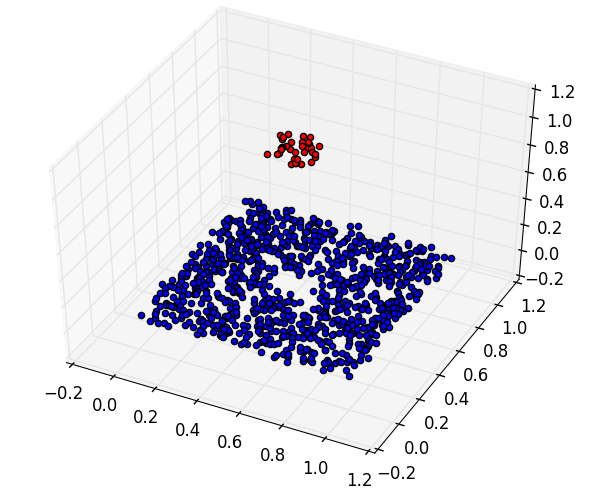
\includegraphics[width=0.6\linewidth]{img/test0.png}
    \caption{Dane testowe w rzucie 3D}
    \label{fig:dane_zerowe}
\end{figure}

Dane testowe oraz wyniki działania algorytmu przedstawiono na rysunkach \ref{fig:test1} i \ref{fig:test2}.
Przez kolor czerwony zostały oznaczone punkty dla których $z > 1$.

\begin{figure}[h!]
    \centering
    \begin{subfigure}[b]{0.5\linewidth}
        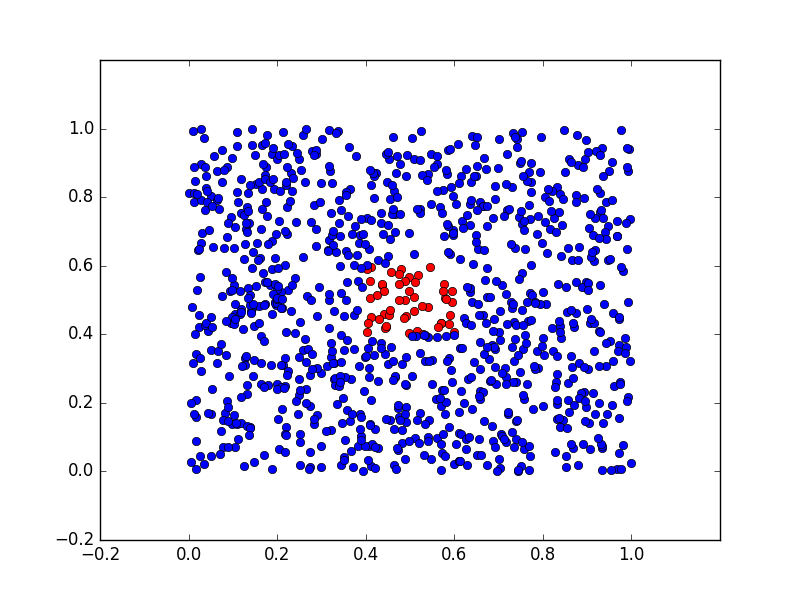
\includegraphics[width=\linewidth]{img/test1_1.png}
		\caption{Dane wejściowe}
    \end{subfigure}%
    \begin{subfigure}[b]{0.5\linewidth}
        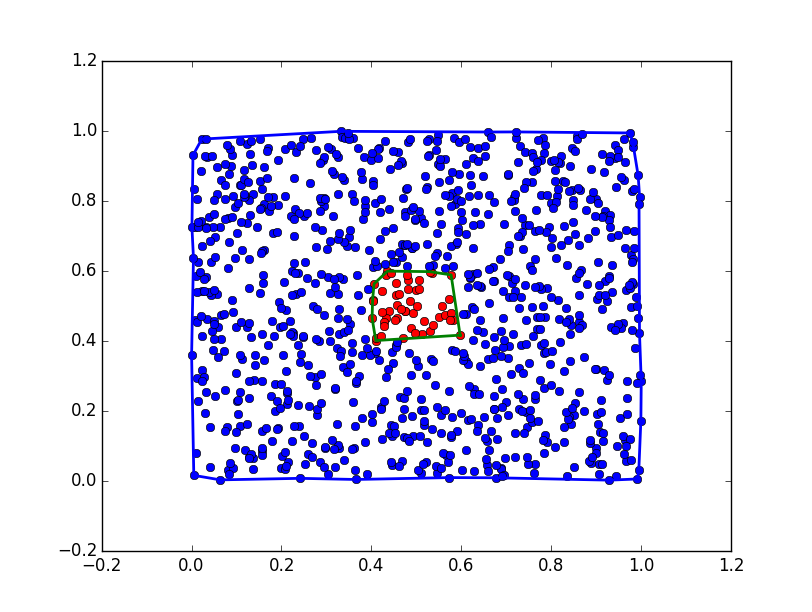
\includegraphics[width=\linewidth]{img/test1_2.png}
		\caption{Algorytm naiwny}
    \end{subfigure}%

    \begin{subfigure}[b]{0.5\linewidth}
        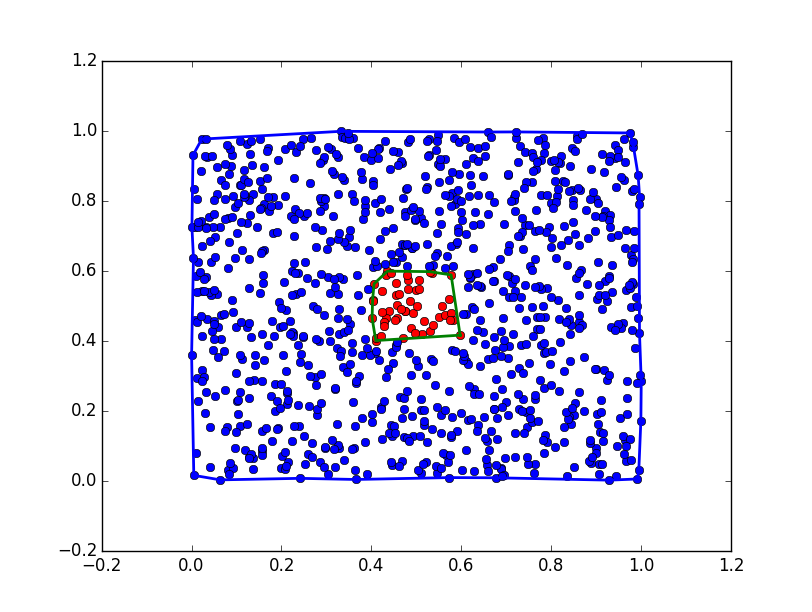
\includegraphics[width=\linewidth]{img/test1_3.png}
        \caption{Algorytm iteracyjny (1 iteracja)}
    \end{subfigure}%
    \caption{Wyniki działa algorytmu dla wygenerowanych danych testowych}
    \label{fig:test1}
\end{figure}

Jak widać na rysunku \ref{fig:test1} oba algorytmy poprawnie wykryły dwie powierzchnie. Co ciekawe,
algorytm iteracyjny już po pierwszej iteracji poprawnie zakwalifikował punkty do dwóch zbiorów. Niestety, jest to
dziełem przypadku, co pokazano na rysunku \ref{fig:test2}

\begin{figure}[h!]
    \centering
    \begin{subfigure}[b]{0.5\linewidth}
        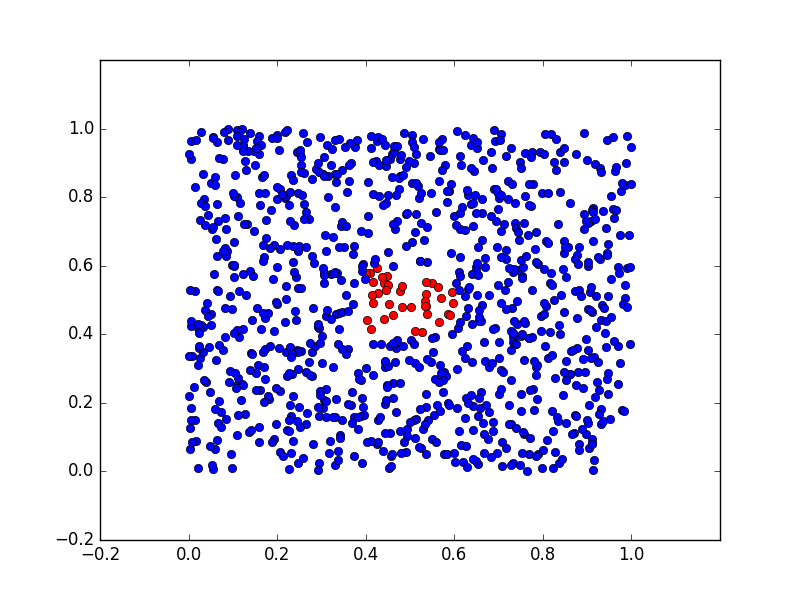
\includegraphics[width=\linewidth]{img/test2_1.png}
        \caption{Dane wejściowe}
    \end{subfigure}%
    \begin{subfigure}[b]{0.5\linewidth}
        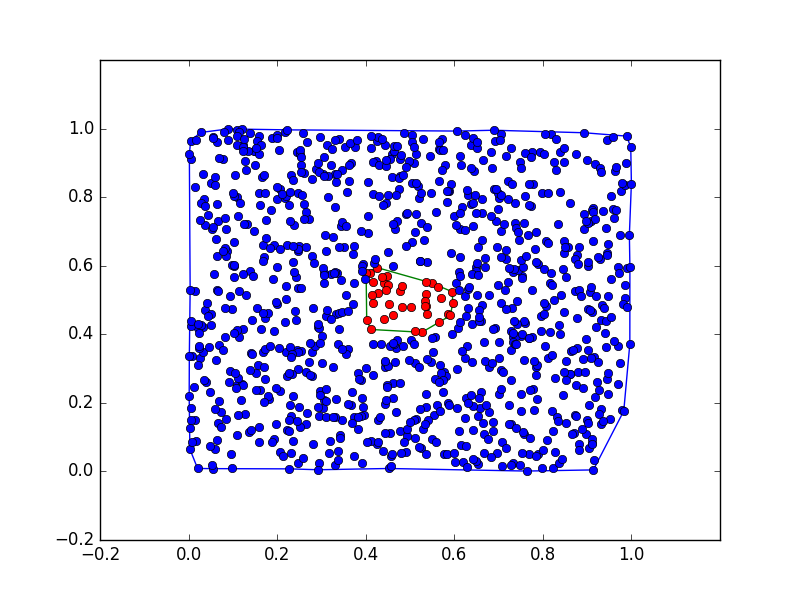
\includegraphics[width=\linewidth]{img/test2_2.png}
        \caption{Algorytm naiwny}
    \end{subfigure}%

    \begin{subfigure}[b]{0.5\linewidth}
        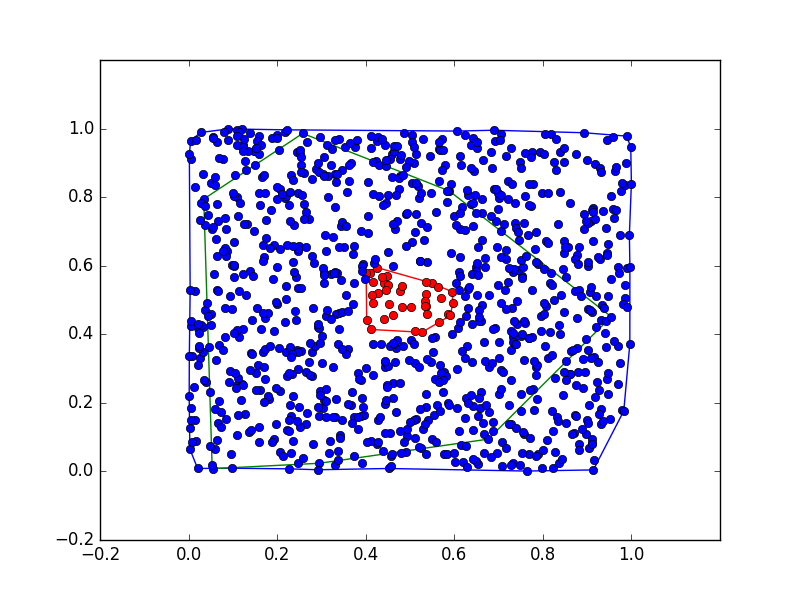
\includegraphics[width=\linewidth]{img/test2_3.png}
        \caption{Algorytm iteracyjny (1 iteracja)}
    \end{subfigure}%
    \begin{subfigure}[b]{0.5\linewidth}
        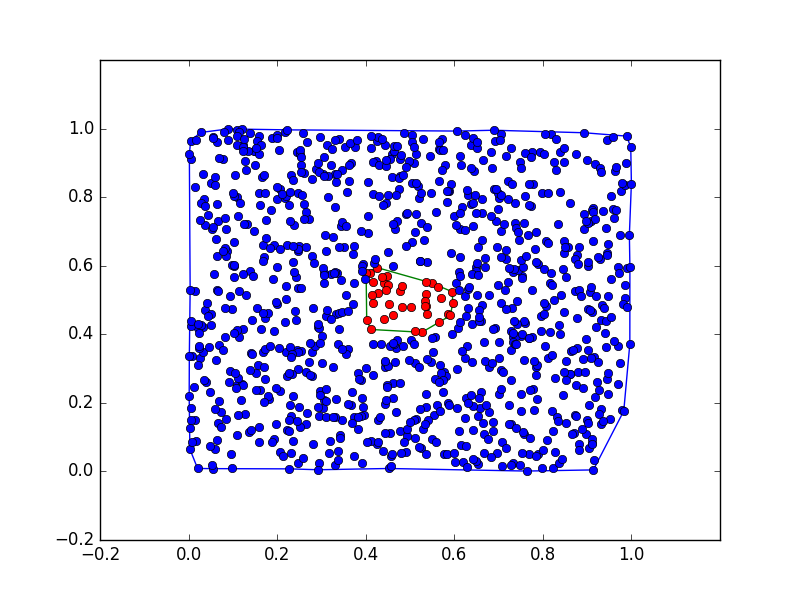
\includegraphics[width=\linewidth]{img/test2_4.png}
        \caption{Algorytm iteracyjny (7 iteracja)}
    \end{subfigure}%
    \caption{Wyniki działa algorytmu dla wygenerowanych danych testowych}
    \label{fig:test2}
\end{figure}

W przypadku pokazanym na rysunku \ref{fig:test2} koniecznych było 7 iteracji, aby w prawidłowy sposób wykryć, iż
w danych testowych znajdują się dwie powierzchnię. Przypadek ten pokazuje, że algorytm iteracyjny ma właściwości
poprawiania wyników wraz z kolejnymi iteracjami. Porównano także czasy wykonywania się algorytmów (tabela \ref{tab:czasy1})

\begin{table}[h!]
    \centering
    \begin{tabular}{|p{0.5\linewidth}|p{0.5\linewidth}|}
        \hline
        Algorytm Naiwny & 1,40s \\
        \hline
        Algorytm Iteracyjny - 1 iteracja & 15,47s \\
        \hline
        Algorytm Iteracyjny - 7 iteracji & 4min 33,08s (273,08s) \\
        \hline
        Algorytm Iteracyjny - 7 iteracji (średni czas 1 iteracji) & 39,01s \\
        \hline
    \end{tabular}
    \caption{Średnie czasy wykonywania sie algorytmu}
    \label{tab:czasy1}
\end{table}





\listoffigures
\addcontentsline{toc}{chapter}{Spis rysunków}
\listoftables
\addcontentsline{toc}{chapter}{Spis tabel}


\bibliographystyle{unsrt}
\bibliography{bibliografia}

%*****************
%\begin{appendices}
%\chapter{Derivation of Pipe-flow Process Model}

Since the derivation of the model is based on physical relationships and conservation principles it would be convenient to study at least once the consecutive steps performed in order to obtain it. This may provide reader with better understanding of the process as well as present assumptions and approximations that are utilized. The model is derived starting from two equations: equation of continuity and equation of motion. The derivation provided below is based on \cite{billmann_isermann,keerthi_phd}.

\section{Equation of Continuity}

We start from definition of the mass:

\begin{equation}
\label{eq:mass}
m = \rho A \Delta z
\end{equation}

Considering mass change in time, i. e. mass-flow

\begin{equation}
\label{eq:massflow}
q = \frac{\partial m}{\partial t} = \rho A  w
\end{equation}

and then, introducing principle of conservation for elementary pipe segment we obtain

\begin{equation}
\label{eq:massflow2}
\frac{\partial m}{\partial t} = \rho A w - A\left(w + \frac{\partial w}{\partial z}\Delta z\right) \left( \rho + \frac{\partial \rho}{\partial z}\Delta z\right) 
\end{equation}

Substituting (\ref{eq:mass}) to  (\ref{eq:massflow2}) we obtain

\begin{equation}
\label{eq:massflow3}
\frac{\partial \left( \rho A \Delta z \right)}{\partial t} = \rho A  w - A\left( \rho w + \Delta z \left( \rho \frac{\partial w}{\partial z} +w \frac{\partial \rho}{\partial z} \right)+\frac{\partial w}{\partial z} \Delta z  \frac{\partial \rho}{\partial z} \Delta z  \right) 
\end{equation}

where the last term $\frac{\partial w}{\partial z} \Delta z  \frac{\partial \rho}{\partial z} \Delta z$ is small enough to be neglected. Then, substituting

\begin{equation}
\label{eq:ms4}
\rho \frac{\partial w}{\partial z} +w \frac{\partial \rho}{\partial z} = \frac{\partial}{\partial z} \left( \rho w \right)
\end{equation}

as

\begin{equation}
\label{eq:ms5}
\frac{\partial}{\partial z} \left( \rho w \right) + \frac{\partial \rho}{\partial t} = 0
\end{equation}

Assuming, that the process is isothermal we can introduce

\begin{equation}
\label{eq:ms6}
\nu = \sqrt{\frac{p}{\rho}}
\end{equation}

thus, substituting (\ref{eq:massflow}) and (\ref{eq:ms6}) to (\ref{eq:ms5}) we obtain first equation of our model:

\begin{equation}
\label{eq:cont_fin3}
\frac{A}{\nu^2} \frac{\partial p}{\partial t} + \frac{\partial q}{\partial z} = 0
\end{equation}


\section{Equation of Motion}

Here we start from definition of momentum:

\begin{equation}
\label{eq:mm1}
M = \rho A \Delta z w
\end{equation}

then,using principle of conservation:

\begin{equation}
\label{eq:mm2}
\frac{\partial \left( \rho A w \Delta z \right)}{\partial t} = A \left(p + \frac{\rho w^2}{2} \right) - A\left(p + \frac{\partial p}{\partial z} \Delta z + \frac{\rho w^2}{2} + \frac{\partial}{\partial z} \left( \frac{\rho w^2}{2} \right) \Delta z \right) - F - Y
\end{equation}

By rearranging equation presented above, we obtain:

\begin{equation}
\label{eq:mm3}
\frac{\partial \left( \rho A w \Delta z \right)}{\partial t} = A \left(p + \frac{\rho w^2}{2} \right) - A\left(\left(p + \frac{\rho w^2}{2} \right) + \Delta z \left( \frac{\partial p}{\partial z} +  \frac{\partial}{\partial z} \left( \frac{\rho w^2}{2} \right) \right)\right) - F - Y
\end{equation}

Substituting 

\begin{equation}
\label{eq:mm4}
 \frac{\partial}{\partial z} \left(p +  \frac{\rho w^2}{2} \right) = \frac{\partial p}{\partial z} +  \frac{\partial}{\partial z} \left( \frac{\rho w^2}{2} \right) 
\end{equation}

into (\ref{eq:mm3}) we will obtain
\begin{equation}
\label{eq:mm5}
\frac{\partial \left( \rho  w  \right)}{\partial t} = -  \frac{\partial}{\partial z} \left(p +  \frac{\rho w^2}{2} \right) - F- Y
\end{equation}

Again, assuming that the process is isothermal we obtain:

\begin{equation}
\label{eq:mm_fin}
\frac{1}{A} \frac{\partial q}{\partial t} + \left( 1 - \frac{q^2 \nu^2}{2 A^2 p}\right) \frac{\partial p}{\partial z} + \frac{q \nu^2}{A^2 p} \frac{\partial q}{\partial z}= - \frac{\lambda \nu^2}{2DA^2} \frac{q|q|}{p} - \frac{g sin \alpha}{\nu^2} p
\end{equation}

Taking into account, that if $w^2 \ll \nu^2$, i. e. velocity of the fluid is significantly lower than velocity of the sound in this fluid, we may neglect term $ \frac{q^2 \nu^2}{2 A^2 p}$. Moreover, if the pipeline is long, then we may neglect term $ \frac{q \nu^2}{A^2 p}$. Thus, we obtain second equation that is included in physical, continuous time model:

\begin{equation}
\label{eq:momen_fin3}
\frac{1}{A} \frac{\partial q}{\partial t} + \frac{\partial p}{\partial z} = - \frac{\lambda \nu^2}{2DA^2} \frac{q|q|}{p} - \frac{g sin \alpha}{\nu^2} p
\end{equation}

%\chapter{CD-ROM Content and Application Structure}

CD-ROM contains $\mbox{MATLAB}^{\mbox{\textregistered}}$ .m files that were developed while working on this thesis. In the main directory there is .pdf file with electronic version of this work. In the folder "sourcecode" there are following files:

\begin{itemize}
\item \textbf{wyzn2.m, wyznacznik.m} - files that were used to check whether determinant of recombination matrix has been properly calculated.
\item \textbf{accuracy3.m} - file used for evaluating accuracy of compared methods.
\item \textbf{kka\_accuracy\_norm.m} - file used for comparison of norms of residual matrices.
\item \textbf{pipe\_simulator.m, sym\_rur\_di.m} - both files were used to model leak and then check the models if they are able to produce correct estimates of leak size and location. Former one needs latter to work properly.

\end{itemize}

\section{Programming Environment and Program Description}

As stated above, all programs are in the form of $\mbox{MATLAB}^{\mbox{\textregistered}}$ files and are intended to work with this environment. In first position listed above is program for given matrix computes its determinant. Latter two positions consists of more complex programs, where the inversion of matrix is conducted using methods introduced earlier, where the methods are described in chapter 3. The last position on the list is the core part of the thesis that helps to evaluate the validity of the models, thus it is described briefly in following section.

\section{Pipe Simulator Application}

In order to check, whether the models produces proper results, the results are compared with the ones given by the model described in \cite{keerthi_phd}. General scheme of application is presented on figure \ref{fig:appl_scheme}.

\begin{figure}[ht]
   \centering
   \includegraphics[scale=0.75]{img/ldi_prog_scheme3.png}
   \caption{Scheme of pipe simulator used to evaluate validity of obtained results.}
\label{fig:appl_scheme}
\end{figure}

Application consists of two main subprograms: pipe simulator and leak detection and isolation.

\subsection{Pipe Simulator Program}

First subprogram is based on description provided in chapter 4. First step is to initialize the the pipe based on provided in program initial conditions, leak parameters and physical specification. From the initial conditions the state space model is constructed as in (\ref{eq:stan_pref5}). After the initialization there is a phase of simulation, where the values of $\hat{Q}_{in}, \hat{Q}_{ex}, \hat{P}_{in}$ and $\hat{P}_{ex}$ are determined. The data produced by that subprogram is treated as input data for leak detection and isolation system.

\subsection{Leak Detection and Isolation}

Second subprogram uses the data generated by pipe simulator. At first, there is an initialization to obtain state space model of pipe flow process with the same parameters as in pipe simulator. Further, the inversion of matrices is conducted using two methods introduced in chapter 3. After inversion three models are constructed and simulated in order to obtain estimates of inlet and outlet signals. After determination of these signals, the residuals are generated and processed in order to obtain the parameters of the leak.

\section{Application Manual}

To use the program, please open file "pipe\_simulator.m" it using $\mbox{MATLAB}^{\mbox{\textregistered}}$ version 7.0 or later. To specify the parameters of the pipe, its physical parameters can be changed by editing lines 10 to 20, where $Nd$ is number of the segments, $L$ length of the pipe, $c$ velocity of the sound, $Tl$ time of the leak, $Tr$ rise time of the leak, $zl$ location of the leak and $ql$ size of the leak. All values should be given in basic SI unit. Also, there is a possibility to change the number of simulation steps in line 3. After specification of physical parameters, press F5 button to start the simulation. In the main window of the program there will be information after every 1000 steps. At the end of pipe simulator subprogram the leak detection and identification part will be executed. After the simulation, the leak estimates are displayed in the form of figures. Each figure is properly labeled.

%\end{appendices}
%*****************

\end{document}
